\documentclass[]{article}
\usepackage[czech]{babel}
\usepackage[utf8]{inputenc}
\usepackage{float}
\usepackage{subfig,graphicx}
\usepackage{array}

\newcommand{\ptheory}{$\Psi$-theory}

\begin{document}

\title{Kapitola 5: Využití metodologie DEMO pro vytváření BPMN modelů}
\author{Bc. Štěpán Heller}
\date{\today}
\maketitle

\section{Motivace} \label{sec:motivace}
Tato kapitola se zabývá přístupy, jak využít silných stránek metodologie DEMO pro vytváření BPMN modelů. Cílem těchto přístupů je vytvořit modely podnikových procesů v BPMN, které budou splňovat stejné požadavky, jaké klade metodologie DEMO. Tedy, že modely musí být ucelené, konzistentní, úplné, výstižné a obsahují jen nezbytné množství informací. Jak píše \cite{VanNuffel2009}, BPMN začíná tam, kde DEMO končí, tedy by se mohlo zdát, že je vhodné jejich silné stránky spojit.

\subsection{Slabé stránky DEMO}
Jak již bylo v průběhu této práce několikrát zmíněno, na metodologii DEMO je nejcennější, že říká tvůrcům procesních modelů \uv{jak} by měli při vytváření modelů podnikových procesů postupovat a nedává jim tedy pouze notaci, pomocí které je možné to realizovat. Nutno však zároveň říct, že teoretický základ metodologie DEMO (tedy kombinace enterprise ontology a \ptheory) je pro běžného uživatele velmi nepřístupný a obtížný na pochopení, protože jeho základy sahají až k fundamentálním filozofickým konceptům, jakými právě ontologie jsou. 

Křivka učení je tedy v tomto případě velmi pozvolná a k plnému pochopení metodologie DEMO je potřeba hodně času a zkoušení metodou pokus-omyl. Autor této práce má zkušenosti z účasti na kurzu MI-MEP (Modelování ekonomických procesů) na Fakultě informačních technologií ČVUT, kde po dobu jednoho semestru bylo certifikovanými DEMO profesionály vyučováno DEMO po teoretické i praktické stránce. Z autorových zkušeností i po absolvování celého 3 měsíčního kurzu měli jeho účastníci problém se základními technikami metodologie DEMO, jakou je například korektní aplikace distinction axiomu performa-informa-forma analýzou, ale i s dalšími fundamentálními věcmi.

Nebudeme tedy daleko od pravdy, když konstatujeme, že v případě běžných uživatelů (návrhářů, analytiků, vývojářů) v rámci podniků bude problém podobný. Dalším nedostatkem DEMO je množství nástrojů, které DEMO podporují, kterých je minimum a žádný z nich dosud nepokrývá všechny aspect modely, které DEMO obsahuje. Nutno však říct, že komunita kolem DEMO je velmi aktivní a na vývoji těchto nástrojů se intenznivě pracuje.

Cílem této práce je umožnit takovým uživatelům nadále využívat nástroje, které znají (BPMN) a umí používat, ale v rámci metodologie DEMO identifikovat \uv{nezbytné minimum} z teoretického základu, které zvýší kvalitu výsledných procesních BPMN modelů a tím umožní i jejich lepší analýzu a optimalizaci

\subsection{Slabé stránky BPMN}
U BPMN nacházíme slabiny tam, kde jsme u DEMO indentifikovali silné stránky a naopak. Jak již bylo naznačeno v kapitole 2 velkým problémem BPMN je absence pevného teoretického základu, který dává návrhářům pevný rámec, podle kterého se mohou řídit a vytvářet modely, podle pevně daných pravidel a postupů. Absence takového pevného rámce pak ústí v to, že modely jsou neúplné a chybí v nich podstatné informace nebo v to, že v momentě, kdy různí uživatelé modelují jeden a ten samý proces, tak skončí s různými modely i když jsou všechny dle specifikace BPMN korektní.

Problematické je i absence seznamu pravidel, co který element v BPMN přesně vyjadřuje, kdy ho používat a kdy ne. Popis jednotlivých elementů je rozprostřen na 500 stranách v celé specifikaci BPMN \cite{Silver2011} a uživatelé jsou tak odkázáni na interpretaci této specifikace, která pochází většinou od tvůrců modelovacího nástroje, který tito uživatelé aktuálně používají. To pak dále tříští způsob, jakým jsou elementy používány.

V praxi v organizacích často vidíme, že mezi procesními analytiky a vývojáři přirozeně vzniká jakási pseudo-metodologie, právě z důvodu toho, aby bylo možné uvnitř organizace konzistentně vytvářet modely podnikových procesů stejným způsobem i v týmu více lidí a aby byla zajištěna kontinuita i v případě fluktuace členů tohoto týmu. Jedním z přínosů této práce, by mělo být vytvoření pevného rámce založeného na ontologiích a \ptheory, který by mohl nahradit tyto pseudo-metodologie.

Zajímavá zjištění uvádí \cite{Caetano2012}, kde při svém výzkumu aplikovali zásady, na kterých stojí metodologie DEMO, na dva klíčové procesy ve velké organizaci (více než 2000 zaměstnanců). Tyto procesy obsahovaly dohromady přes 500 aktivit a více než 60 aktorů. Analytici prověřovali, zda je procesní model konzistentní, tedy zda pořadí kroků v tomto procesu odpovídá transakčnímu axiomu. Dále se zajímali, zda je takový model kompletní, neboli jestli všechny kroky transakce dle transakčního axiomu DEMO se dají namapovat na aktivity BPMN modelu. Po důkladné analýze těchto procesů došli k následujícím zjištěním:

\begin{itemize}
\item V původních procesech chybělo 25 \% p-faktů neboli tyto procesy obsahovaly aktivity, které nebylo možné přiřadit k vytváření nějakého výsledku (hmotného či nehmontého).
\item Chybělo rovněž 25 \% request C-actů. Tedy výsledky byly produkovány bez explicitního požadavku na jejich tvorbu a tedy nebylo možné jasně identifikovat iniciátora celé transakce.
\item Chybělo 50 \% promise C-actů. Requesty byly implicitně potvrzovány bez jakékoliv jasné dohody mezi aktory.
\item Chybělo 25 \% state C-actů. Výsledky transakce tak nebyly jasně komunikovány s jejím inicátorem a tedy není jasné, zda dohlídnutí na výsledek transakce leží na iniciátorovi nebo exekutorovi.
\item Chybělo 40 \% accept C-actů. Nebylo tedy možné identifikovat, jak jsou výsledky transakce akceptovány jejím iniciátorem a jestli takové výsledky splňují požadavky, které na ně byly kladeny při requestu.
\end{itemize}

Je tedy zřejmé, že absence pevného teoretického je reálným problémem (ač ho uživatelé sami nepociťují \cite{VanNuffel2009}) a jeho vytvoření by zvýšilo kvalitu vytvářených modelů podnikových procesů.

\subsection{Benefity kombinace DEMO a BPMN}
Hlavním přínosem této práce je vytvoření rámce, který vychází z metodologie DEMO a slouží ke stanovéní základů metodologie, která v budoucnu umožní vytváření kvalitnějších BPMN modelů. Slovo \uv{kvalitnější} si na tomto místě zaslouží hlubší rozebrání.

Cílem této práce není vytvoření metodologie, která bude dokonale kopírovat DEMO a v podstatě jen umožní vytvoření DEMO modelů za použití notace BPMN. Abstrahujme zde od toho, zda je to vůbec možné, to musí být potvrzeno dalším výzkumem. Pokud bychom se k takovému přístupu rozhodli, nedosáhli bychom vyřešení problémů uvedených v předchozí sekci \ref{sec:motivace}. Cílem této práce je nalézt takový teoretický rámec, který bude stále pochopitelný pro uživatele a umožní jim vytvářet kvalitnější BPMN modely, ale nebude s sebou nést dlouhou křivku učení, kterou obsahuje DEMO. Co je tedy míněno \uv{kvalitnějšími} BPMN modely?

\begin{itemize}
\item Modely takto vytvořené budou \textit{kompletní} dle transakčního axiomu, tedy nebude chybět žádný krok dle transakčího axiomu. %možná ne%
\item Modely takto vytvořené budou \textit{jednoznačné}, neboli při modelování toho samého procesu by vždy měl vzniknout ten stejný model
\item Modely budou oproštěné od implementačních detailů a budou tedy zachycovat jen skutečné jádro organizace
\end{itemize}

We consider a process model to be consistent if its activities comply with the business transaction pattern. 

If a process complies with the transac- tion pattern then its specification describes who is responsible for the execution of its activities and why each activity is being performed. However, a business process can be consistent but still be missing activities required to fully produce the intended transactional results. This means that a complete process must not only be consistent but also specify all transactional activities.

A business process model is consistent if the order of its actions complies with the transactional axiom. A business process model is complete if all transactional pattern steps can be mapped to its activities.

Thus, a process model that is both consis- tent and complete is a process that fully specifies an end-to-end collaboration pattern between a service requester and a service provider.

%todo jaké nebudou%

\section{Existující možnosti společného využití obou přístupů} \label{sec:existujici_moznosti}
Vhodnost spojení obou přístupů neušla pozornosti jiných autorů, například \cite{VanNuffel2009}, \cite{Caetano2011} nebo \cite{Caetano2012}. Ve stručnosti budou na tomto místě tyto přístupy popsány, protože i na jejich zjištěních autor této práce svůj návrh metodologie staví.

\subsection{Analýza procesních modelů pomocí $\Psi$-Theory} \label{sec:analyza_proc_modelu_psi}
V \cite{Caetano2012} a \cite{Caetano2011} se autor zabývá využitím $\Psi$-Theory pro analýzu modelů podnikových procesů s cílem zvýšit jejich \textit{kompletnost} a \textit{konzistentnost}. Za tímto účelem představuje autor metodu jejímž vstupem je procesní model v notaci BPMN. Metoda se skládá z následujících čtyř kroků:

\begin{enumerate}
\item Provedení analýzu vstupního BPMN modelu s cílem klasifikovat jednotlivé elementy jako C-act nebo P-act a také rozlišit, zda jsou ontologické, infologické nebo datalogické. Dále je nutné se pokusit v modelu identifikovat Actory odpovědné za vykonání C-actů a P-actů.

Ontologické C-acty jsou následně klasifikovány dle jednotlivých kroků \textit{standardního transakčního vzoru}.
\item V dalším kroku je vygenerován DEMO Process Structure Diagram (PSD) na základě seznamu Actorů, transakcí, C-actů a P-actů získaných v předchozím kroku.
\item Ve třetím kroku je PSD diagram z předchozího kroku doplněn o C-acty a P-acty, které v něm chybí oproti transakčnímu vzoru. Dále je vytvořen DEMO Actor Transaction Diagram (ATD) pro zobrazení návaznosti transakcí dle \textit{Composition axiomu}.
\item V následujícím kroku je provedena revize vstupního BPMN modelu a ten je na odpovídajících místech doplněn o elementy představující chybějící C-acty nebo P-acty identifikované v předchozím kroku. Takto revidovaný vstupní model je nyní \textit{kompletní} a \textit{konzistentní} dle $\Psi$-Theory.
\end{enumerate}

Opakovanou aplikací této metody za účasti doménových i procesních vlastníků je možné dosáhnout procesních modelů, které uspokojí business uživatele a zároveň budou \textit{kompletní} a \textit{konzistentní} dle $\Psi$-Theory. Iterativní způsob aplikace představené metody ilustruje obrázek \ref{fig:caetano-bpmn-demo-method}.

\begin{figure}[H]\centering
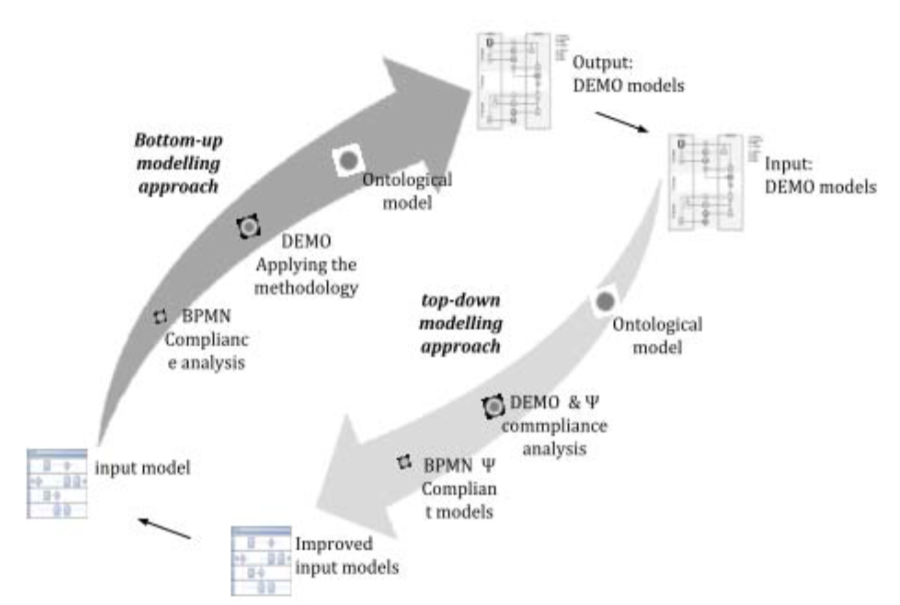
\includegraphics[width=\textwidth,height=\textheight,keepaspectratio]{obrazky/caetano-bpmn-demo-method}
\caption{Iterativní aplikace metody dle \cite{Caetano2011}}
\label{fig:caetano-bpmn-demo-method}
\end{figure}

\subsection{Rozšíření formálních základů BPMN pomocí Enterprise Ontology}

Práce \cite{VanNuffel2009} nazvaná \textit{Enhancing the Formal Foundations of BPMN by Enterprise Ontology} se na teoretické úrovni zabývá možností, jak využít Enterprise ontology jako ontologický základ pro vytváření BPMN modelů a argumentuje, že fundamentální koncepty BPMN jsou \uv{podobné} konceptům DEMO:

\begin{itemize}
\item Koncept \textit{aktivity} je \uv{podobný} konceptu výkonu (performance) nebo DEMO P-factu nebo určité komunikaci o tomto výkonu neboli DEMO C-factu.
\item Koncept \textit{plavecké dráhy} je \uv{podobný} konceptu Actora (Actor-Initiator nebo Actor-Executor)
\end{itemize}

Na tomto základě a následnou důkladnou analýzou axiomů \ptheory autoři došli k 14 pozorováním. Jelikož jsou tato pozorování jedním ze základních stavebních kamenů metodologie navrhované v této práci budou zde uvedeny:

\begin{itemize}
\item Existují identifikovatelní actoři plnící role, kde se actor vztahuje k roli a nikoli nutně k jedinci, který tu roli fyzicky vykonává
\item Existují identifikovatelné P-facty reprezentující nějaký úkon
\item Existují C-facty reprezentující komunikaci o konkrétním úkonu, který má být vykonán
\item Každý P-fact je vztažen pouze k jednomu unikátnímu C-factu a naopak
\item Každý aktor vyjma kořenového actor-initiator má jeden a pouze jeden vztah actor-executor k jednomu a pouze jednomu P-factu, ale může mít $0...n$ actor-initiator vztahů k jiným (child) P-factům.
\item Každý P-fact může být definován jako množina $0...n$ jeho potomků %todo bullshit alert%
\item U každého rodičovského P-factu musí nejdřív dojít k dokončení (state and accept) child P-factů dříve než může začít exekuce rodičovského P-factu.
\item Actor, který je exekutorem nějakého P-factu je zároveň iniciátorem každého jeho child P-factu.
\item Pouze iniciátor kořenového P-factu není iniciátorem žádného jiného P-factu.
\item U každého modelu existuje alespoň jeden P-fact, který je ve vztahu k actorovi, který je pouze exekutorem tohoto P-factu.
\item Existuje množina osmi atributů (Request, Promise, etc.), které se unikátně vztahují ke konkrétnímu C-factu, která  popisuje aktuální stav komunikace ohledně úkonu (vytvoření P-factu).
\end{itemize}

Autoři ve své práci představují nástin dvou přístupů, jak využít DEMO a Enterprise Ontology pro vytváření či vylepšení BPMN modelů. Jedním z přístupů je analýza a doplnění existujících BPMN modelů na základě čtyř základních axiomů \ptheory v základu podobně jak bylo popsáno v sekci \ref{sec:analyza_proc_modelu_psi}. 

Pro tuto práci přínosnější je fakt nástin druhé možnosti – vytváření nových BPMN modelů na formálním základě, který z DEMO a Enteprise Ontology vychází. Vytváření takového BPMN modelu začíná sběrem informací o organizaci, jejím chodu a funkci. Dalším krokem je aplikace \textit{Distinction axiomu} a  vyřazení všech informací, které nejsou ontologické. Třetím krokem je pak ve zbylých informacích nalézt ontologické transakce a Actory, kteří vystupují v rolích Actor-Initiator a Actor-Executor ve vztahu k těmto transakcím. Závěrečným krokem je pak vytvoření DEMO Actor-Transaction Diagramu, který zobrazuje vztah mezi transakcemi a Actory. 

Výsledkem tohoto postupu tedy není BPMN model, ale kroky v něm nastíněné je nezbytné provést, aby bylo možné vytvořit BPMN model, který je \textit{konzistentní} a \textit{kompletní}. Metodologie nastíněná v této práci právě na těchto krokech staví a posouvá je směrem ke skutečnému BPMN modelu.

\section{Návrh metodologie}
\subsection{Výchozí předpoklady}
Důkladným studiem notace BPMN i metodologie DEMO bylo vypozorování několik výchozích předpokladů, které navazují na pozorování dle \cite{VanNuffel2009}, která jsme uvedli v sekci \ref{sec:existujici_moznosti}.

\begin{itemize}
\item V notaci BPMN nenajdeme žádné transakce tak, jak je definuje DEMO. Ve verzi BPMN 2.0 sice konstrukt nazvaný transakce existuje, ale v tomto případě se jedná pouze o speciální druh elementů, který vyžaduje definici kompenzačních aktivit v případě, že je nutné transakci odvolat.
\item
\end{itemize}

\subsection{Základní pravidla používání notace BPMN} \label{sec:zakladni_pravidla}
V této sekci jsou vypsány základní pravidla, jak používat některé elementy z notace BPMN tak, aby jejich použití korespondovalo s vybranými konstrukty z metodologie DEMO dle konceptu metodologie představené v této práci. Z metodologie DEMO byly vybrány zejména ty koncepty, které jsou součástí transakčního axiomu, který je pro vlastní tvorba modelů podnikových procesů nejzásadnější a vyjádření tohoto axiomu pomocí korespondujících elementů BPMN by výrazně přispělo k možnosti vytvářet kvalitnější modely v této notaci.
\subsubsection{Vyjádření Actorů}
\textit{Actor} je v DEMO definován jako kombinace odpovědnosti a kompetence a není nezbytně svázán s konkrétním jedincem, který ve výsledku aktivitu či transakci fyzicky provádí. Pokud chceme v BPMN transakce zobrazovat, musí se podařit v paletě elementů, které BPMN nabízí nalézt takové, pomocí kterých je možné aktory korektně vyjádřit. Vybraný element musí splňovat tyto předpoklady:

\begin{itemize}
\item Musí jasně určovat, které kroky transakčního axiomu (C-acty a P-acty) patří do pole zodpovědnosti daného Actora
\item Musí umožňovat komunikaci s druhým Actorem v transakci
\item Musí umožňovat navazování dalších Actorů a transakcí v transakčním stromu
\end{itemize}

Pro znázornění Actora se nabízí využití BPMN elementu \textit{plavecká dráha (swimlane)}. BPMN nijak konkrétně nespecifikuje, jak plavecké dráhy využívat a nechává to tedy v rukou osoby, která model vytváří \cite{Silver2011}. Pro znázornění dvou Actorů v transakci by pak sloužily dvě sousedící \textit{plavecké dráhy}. Komunikace mezi nimi by pak probíhala především pomocí \textit{sekvenčních toků}.

Další možností, jak reprezentovat Actora, je teoreticky \textit{bazén}, který by tak fungoval samostatně pro každého actora a jelikož standard notace BPMN 2.0 zakazuje, aby sekvenční toky překročily hranice bazénu, museli by actoři mezi sebou koordinovat kroky (C-acty, P-acty) pomocí zasílání zpráv. A právě zde tkví hlavní úskalí tohoto přístupu. V odborné literatuře (například \cite{Silver2011}) je obecně uváděno, že není dobrým přístupem modelovat aktivity v rámci jednoho procesu uvnitř více bazénů. Vznikají pak problémy v navazování posloupnosti aktivit na sebe, ale i s korektností výsledného BPMN modelu dle zásad DEMO neboť využití bazénů nám rozdělí transakci fakticky do dvou procesů, což přináší problémy, které budou popsány v. %todo odkaz% 

\subsubsection{Vyjádření C-actů a P-actů}
\textit{C-acty} a \textit{P-acty} jsou jednotlivé kroky v transakčním vzoru, které jsou prováděny v definovaném pořadí a jsou v transakci vždy přítomny, i když jsou někdy prováděny mlčky. Pro vyjádření C-actů a P-actů tato metodologie používá BPMN element \textit{Úlohy (Task)}, který je dále nedělitelným typem \textit{Aktivity}. Úlohy mohou být dále rozlčleněny na ty, které provádí člověk, které systém nebo nějaký stroj atp. Pro účely modelování popsané v této práci se nejlépe hodí abstraktní Úlohy, které jsou bez označení. 

Second, C-acts may be performed tacitly. This means that there is no act at all that counts as performing the C-act. Tacitly performing a C- act, however, is still performing that C-act.

\subsubsection{Vyjádření C-factů}
\textit{C-fact} neboli \textit{coordination fact} je výsledkem provedení \textit{C-actu}. Je tedy přímo navázán na C-act, který jej \uv{vytváří}. V BPMN lze C-fact vyjádřit třemi způsoby:

\begin{enumerate}
\item C-fact explicitně v modelu není vyjádřen. Jeho existence je zajištěna implicitně pomocí \textit{Sekvenčních toků} vycházejících z \textit{Úloh}, které reprezentují C-act.
\item C-fact je vyjádřen pomocí \textit{Signálu}. Důvod pro použití elementu Signál je ten, že druhý Actor by měl být o vzniku C-factu (respektive změně \textit{C-worldu}) informován, což první způsob, ve kterém je to předpokládáno implicitně, nezaručuje.
\item C-fact je vyjádřen pomocí \textit{Zprávy}, kterou zašle Actor, který příslušný C-act vykonal druhému Actorovi.
\end{enumerate}

This C-fact is drawn between the two actor roles to show that it is a fact in their social or intersubjective world ([32]): both actors are allowed to know the fact. 

\subsubsection{Vyjádření P-factů}
Podobně jako \textit{C-fact} je i \textit{P-fact} výsledkem provedení konkrétního \textit{P-actu}. V transakci se objevuje pouze jednou a zjednodušeně lze říci, že je \uv{výsledkem} celé transakce. P-fact může být hmotné povahy (např. upečení pizzy), ale i nehmotné (např. rozhodnutí poroty). Metodologie, která je nastíněna v této práci, P-fact v modelu BPMN explicitně neuvádí. Důvody pro toto rozhodnutí jsou následující:

\begin{itemize}
\item Korespondující P-act (vyjádřený \textit{Úlohou}) nazvaný \textit{Execute} a \textit{Sekvenční tok} z něj vycházející už sami o sobě vyjadřují vznik P-factu.
\item Actor-Iniciátor je o vzniku P-factu informován ve chvíli, kdy je mu předložen pomocí C-actu \textit{State}, který dle transakčního axiomu nastane vždy.
\item Ve standardním i základním transakčním vzoru v metodologii DEMO je P-act i P-fact uváděn pouze v rámci agendy patřící Actorovi-Exekutorovi.
\end{itemize}

\subsubsection{Vyjádření Agendy}

\begin{quote}
Slovo \uv{agenda} vyjadřuje \uv{co musí být uděláno} neboli agenda je \uv{úkol k vyřešení}. \cite{Dietz2006}
\footnote{The word “agendum” is the singular form of the (plural) Latin word “agenda”. It means: what has to be done. In other words, an agendum is a to-do item. \cite{Dietz2006}}
\end{quote}

V metodologii DEMO nejednají Actoři náhodně, ale každý jejich krok je striktně definován pomocí \textit{action rules} v \textit{Action modelu}. Neboli je jasně řečeno například za jakých okolností se vytvoření P-factu přislíbí (\textit{Promise}) a kdy je nutné Request odmítnout. Agenda dle DEMO je čtveřice parametrů:

\begin{itemize}
\item C-fact, který má být vykonán
\item P-fact, kterého se C-fact týká
\item Čas vztahující se k provedení P-factu
\item Čas, kdy by měl být C-fact vykonán %bullshit alert%
\end{itemize}

Jelikož návrh metodologie, který tato práce popisuje, pracuje pouze s existujícími BPMN elementy, není v tuto chvíli možné kompletní Agendu pomocí nich vyjádřit. Řešením by bylo buď vytvořit vlastní doplňující model podobný Action Modelu DEMO nebo přímo DEMO Action Model. Dalším výzkumem je nutné ověřit, zda je vytvoření takové vrstvy nutné a případně takovou vrstvu vytvořit tak, aby byla připravena pro implementaci v softwarovém nástroji, který by tak umožnil simulaci modelovaného procesu.

Metodologie navrhovaná v této práci si vystačí s částečným zobrazením agendy přímo v BPMN modelu, kterého je docíleno pomocí \textit{Plavecké dráhy} (případně \textit{Bazénu}), \textit{Sekvenčního toku} a časového hlediska. Neboli díky Plavecké dráze nebo Bazénu, který obsahuje elementy, jež spadají do kompetence a odpovědnosti Actora, kterému je Plavecká dráha nebo Bazén příslušná a díky Sekvenčnímu toku, který určuje pořadí provádění jednotlivých \textit{Úloh} daný Actor v každém momentě v čase ví, kterou Úlohu má provést. Pravidla pro vyhodnocení, zda přijmout Request nebo State pro zjednodušení opomíjíme.

\section{Vyjádření transakčního vzoru v BPMN} \label{sec:vyjadreni_trans_vzor}
Pro metodologii, která je nastíněna v této práci je transakční vzor dle transakčního axiomu DEMO tím nejdůležitějším stavebním kamenem. Dává totiž řád a jasnou strukturu tomu, jak popsat podnikový proces, který je dle metodologie DEMO jen uspořádanou strukturou na sebe navázaných transakcí – \textit{transakčním stromem}.

Vyjádření transakčního vzoru pomocí elementů z notace BPMN je tak zcela zásadní pro to, aby mohl být naplněn účel nově vznikající metodologie, kterým je přispět k vytváření BPMN modelů, které budou kompletní a jednoznačné. Jak bylo popsáno v sekci \ref{sec:zakladni_pravidla}, vyjádření jednotlivých komponent transakčního vzoru je možné provést pomocí různých elementů a v této sekci jsou tyto různé přístupy rozebrány do většího detailu. 

\subsection{Vyjádření pomocí Úloh} \label{sec:vyjadreni_ulohy}
Prvním a nejjednoduším přístupem je vyjádřit transakční vzor čistě pomocí \textit{Úloh} a \textit{Sekvenčních toků}. Úlohy jsou použity pro vyjádření \textit{C-actů} a \textit{P-actů}. Sekvenční tok je použit ve více významech:

\begin{itemize}
\item jednak pro určení pořadí provádění jednotlivých C-actů,
\item jednak pro zadávání C-factů do Agendy druhému Actorovi,
\item jednak Sekvenční tok vycházející z každé Úlohy reprezentující C-act reprezentuje úspěšný vznik korespondujícího C-factu.
\end{itemize}

Na obrázku \ref{fig:Zk_trans_ulohy} je zobrazen \textit{základní transakční vzor} pomocí Úloh. \textit{Bazén} slouží pro zastřešení celé transakce a \textit{Plavecké dráhy} oddělují Agendy obou zúčastněných Actorů (Iniciátora a Exektuora). Základní transakční vzor bere v potaz pouze \uv{šťastné scénáře}, takže transakce vždy skončí ve stavu \textit{T1 Accepted}. Všechny C-facty, ze kterých transakce již nikam dál nepokračuje jsou vyjádřeny BPMN elementem \textit{Konečná událost (End event)}.

Obrázek \ref{fig:St_trans_ulohy} zobrazuje \textit{standardní transakční vzor}, tedy kompletní transakci včetně všech \uv{nešťastných scénářů (unhappy paths)}. Oproti základnímu transakčnímu vzoru zde přibyly čtyři \textit{Brány} označující místo, kde Actor musí rozhodnout, jak s Agendou naloží. Rozhodnutí je exkluzivní, tudíž je použita \textit{Exkluzivní brána}.

V tomto zobrazení nejsou zobrazeny žádné C-facty, což je z hlediska DEMO problematické. Ačkoliv jejich vznik vyjadřuje Sekvenční tok vycházející z C-actu, C-fact není explicitně vyobrazen a druhý Actor o něm nemusí vědět, protože v modelu není žádná komunikace zobrazena. Dle \cite{Dietz2006} však oba Actoři mají mít umožněno vědět o vzniku C-factu.

\begin{figure}[H]\centering
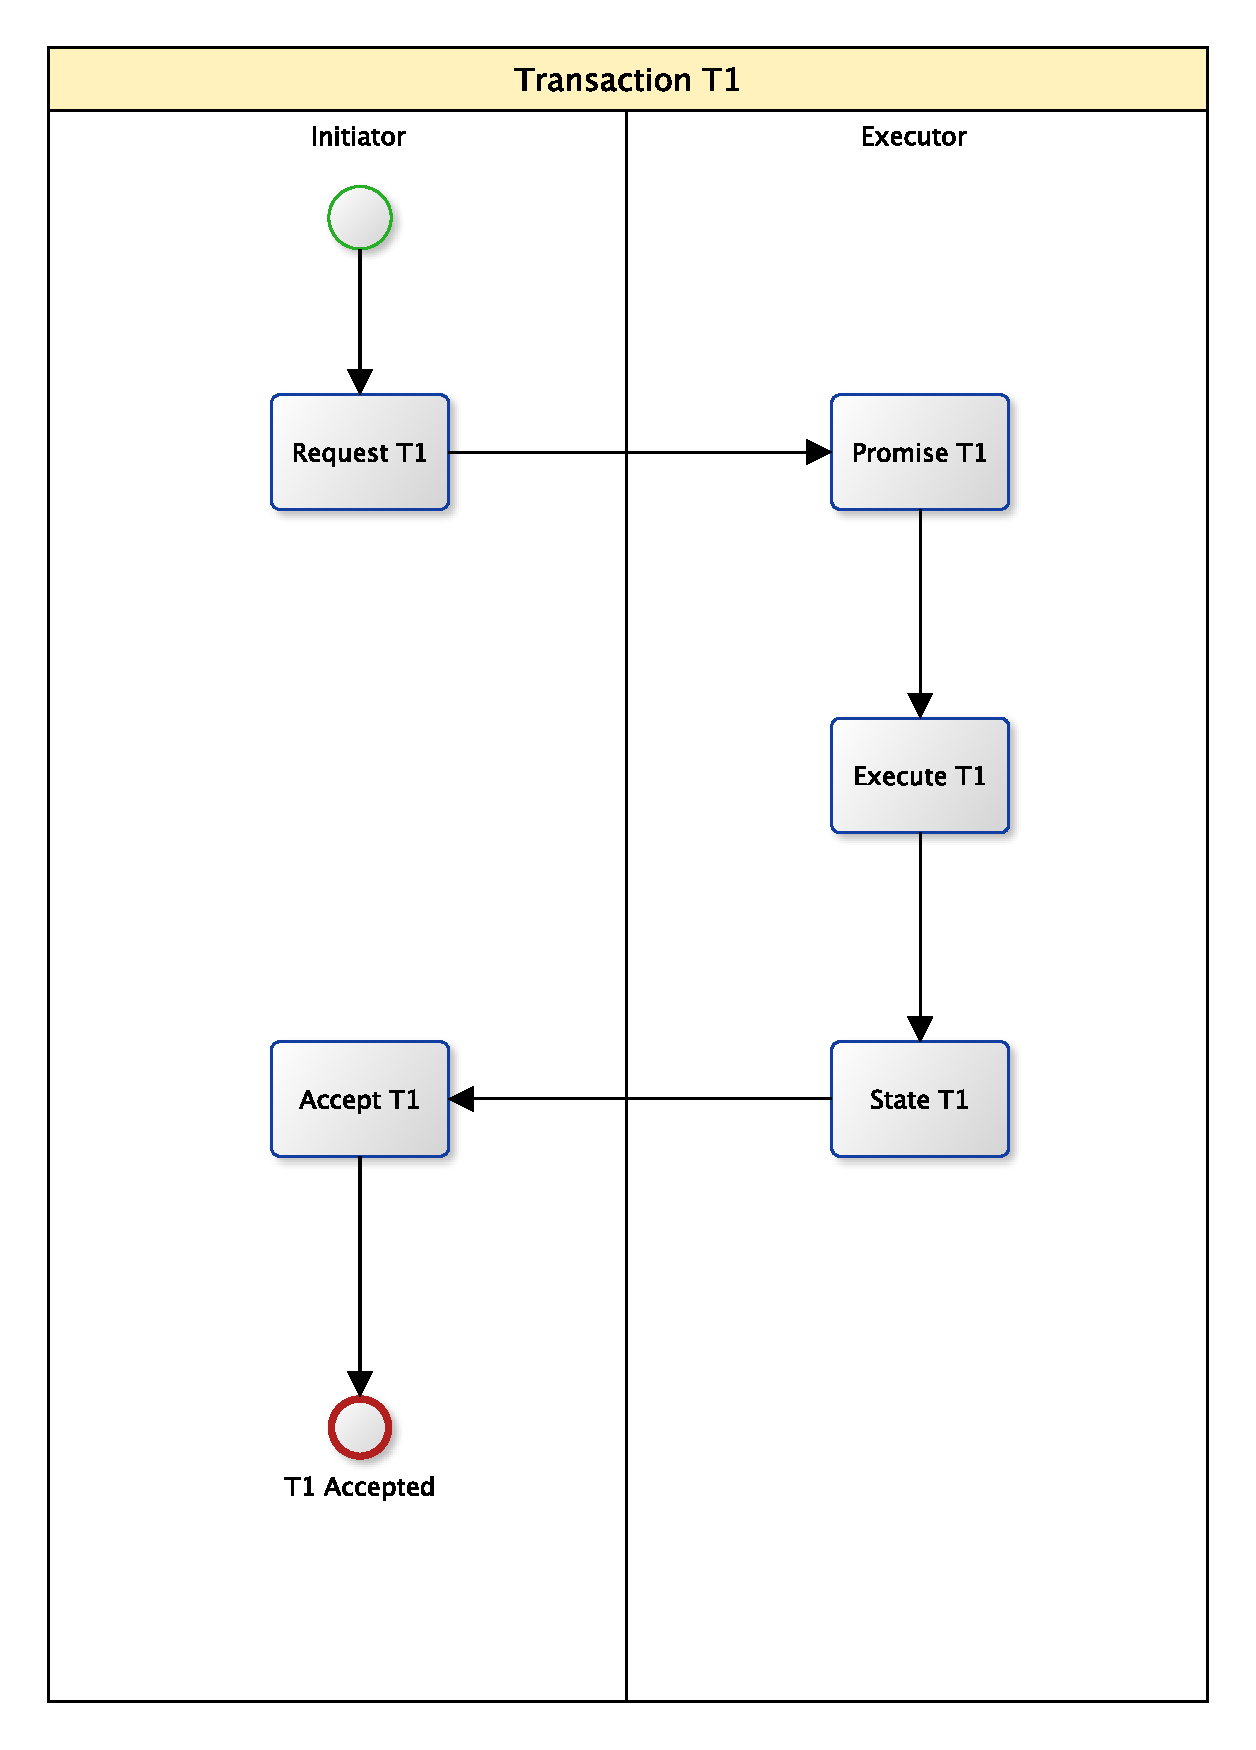
\includegraphics[width=1.0\textwidth]{obrazky/transaction-basic-tasks}
\caption{Základní transakční vzor pomocí Úloh}
\label{fig:Zk_trans_ulohy}
\end{figure}

\begin{figure}[H]\centering
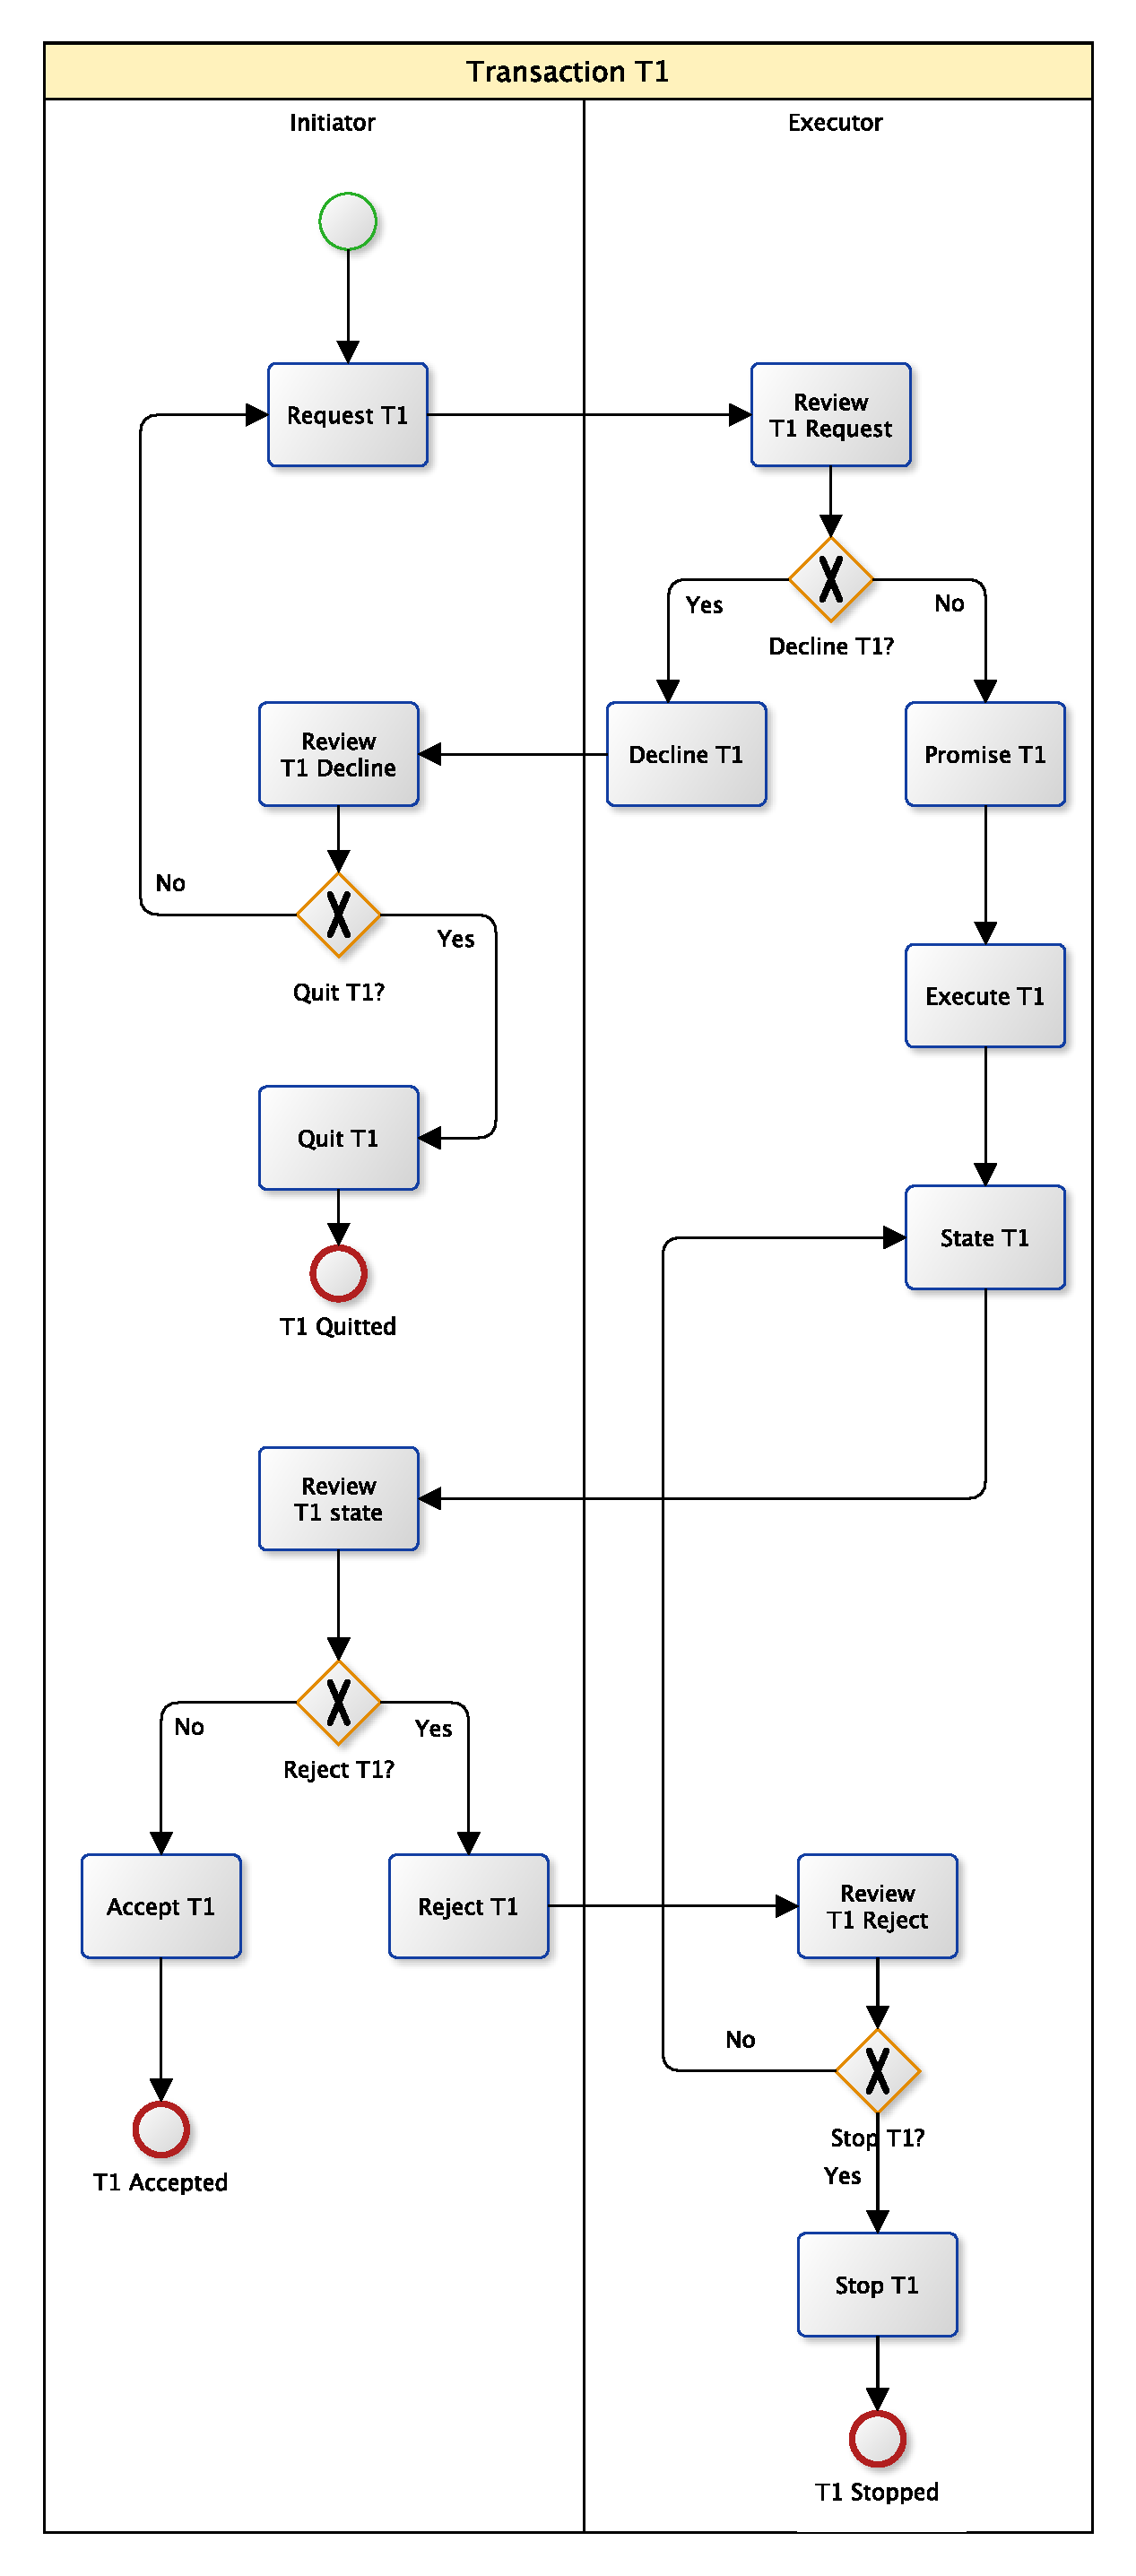
\includegraphics[width=\textwidth,height=\textheight,keepaspectratio]{obrazky/transaction-standard-tasks}
\caption{Standardní transakční vzor pomocí Úloh}
\label{fig:St_trans_ulohy}
\end{figure}

\subsection{Vyjádření pomocí Úloh a Signálů} \label{sec:tr_vzor_ulohy_signaly}

Další možností, jak transakční vzor zobrazit, je využití \textit{Úloh} a \textit{Signálů}. Narozdíl od způsobu popsaného v sekci \ref{sec:vyjadreni_ulohy} \textit{Sekvenční toky} v tomto případě slouží pouze k vyjádření pořadí, ve kterém jsou C-acty prováděny a pro převádění Agendy mezi Actory. O reprezentaci vzniklého C-factu se zde však stará BPMN element Signál, což poskytuje dvě velké výhody. Jednak je díky tomu C-fact v modelu vizuálně zastoupen, takže se výsledný model více blíží transakčnímu vzoru tak, jak ho definuje DEMO a jednak BPMN element Signál, který dle specifikace \cite{Omg2011} i \cite{Silver2011} je možné použít ke komunikaci uvnitř procesu, respektive k odeslání neadresné zprávy komukoliv, kdo je připraven jí naslouchat. Pro reprezentaci Actorů jsou v tomto případě opět použity \textit{Plavecké dráhy} uvnitř \textit{Bazénu}, který zastřešuje celou transakci. C-facty, ve kterých transakce končí jsou i v tomto případě zastoupeny pomocí BPMN elementu \textit{Konečná událost}.

Na obrázku \ref{fig:Zk_trans_ulohy_signaly} vidíme \textit{základní transakční vzor} pomocí Úloh a Signálů. Lze vidět, že po provedení C-actu \textit{Request T1} se Sekvenční tok přesouvá do Signálu \textit{T1 Requested}, který vyjadřuje vzniklý C-fact. Předpokládáme, že Actor-Executor tomuto Signálu naslouchá a může tak provést C-act \textit{Promise T1}.

Obrázek \ref{fig:St_trans_ulohy_signaly} zobrazuje \textit{standardní transakční vzor} vyjádřený Úlohy a Signály.

\begin{figure}[H]\centering
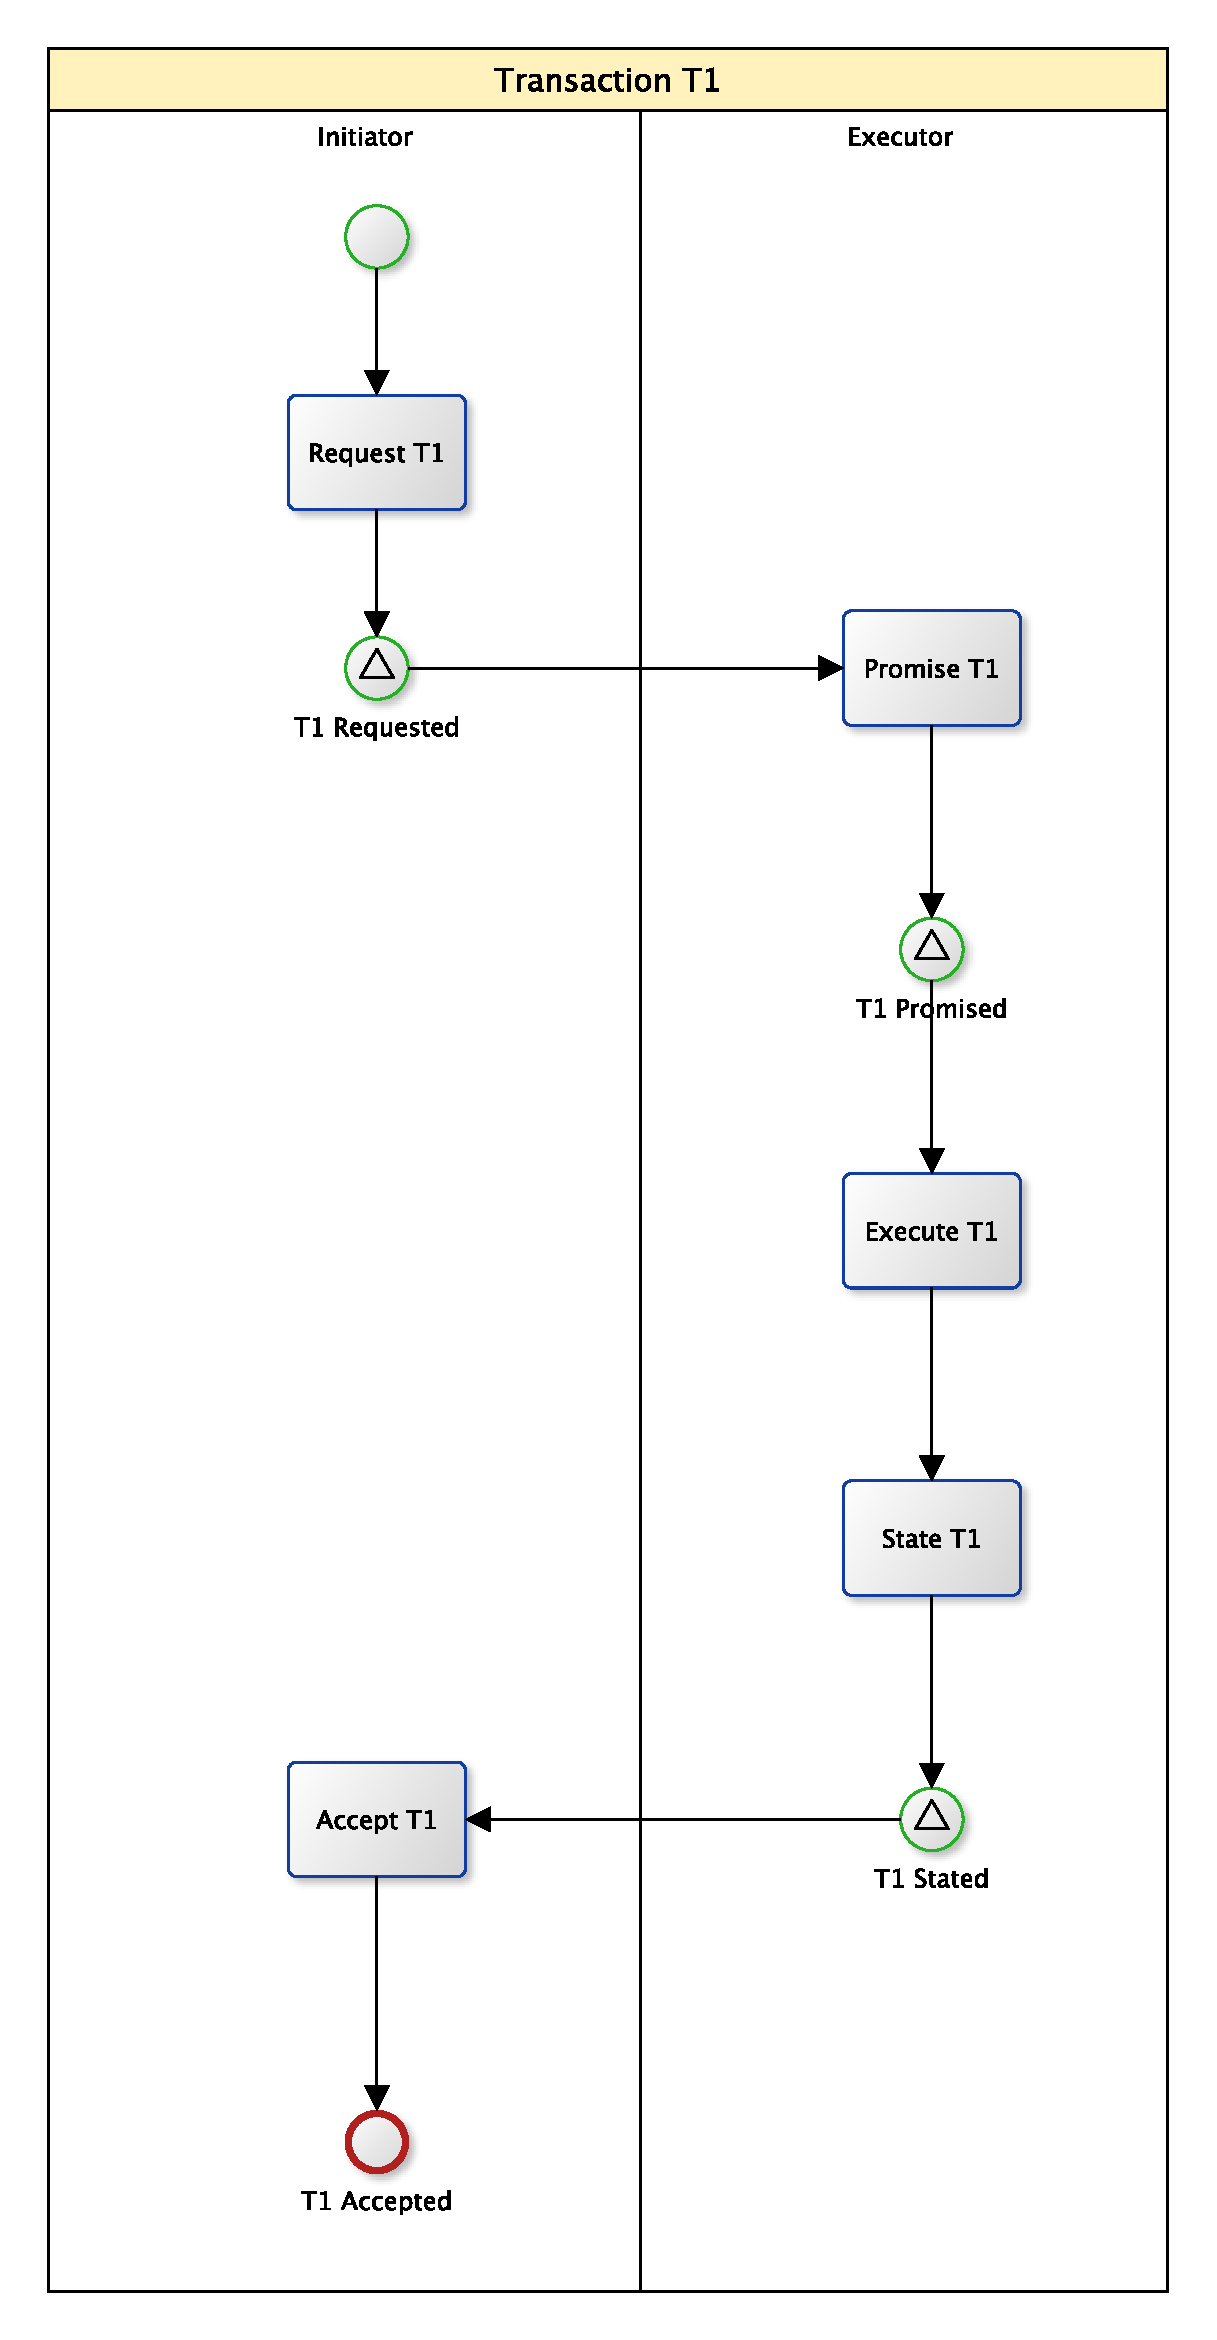
\includegraphics[width=\textwidth,height=\textheight,keepaspectratio]{obrazky/transaction-basic-signals}
\caption{Základní transakční vzor pomocí Úloh a Signálů}
\label{fig:Zk_trans_ulohy_signaly}
\end{figure}

\begin{figure}[H]\centering
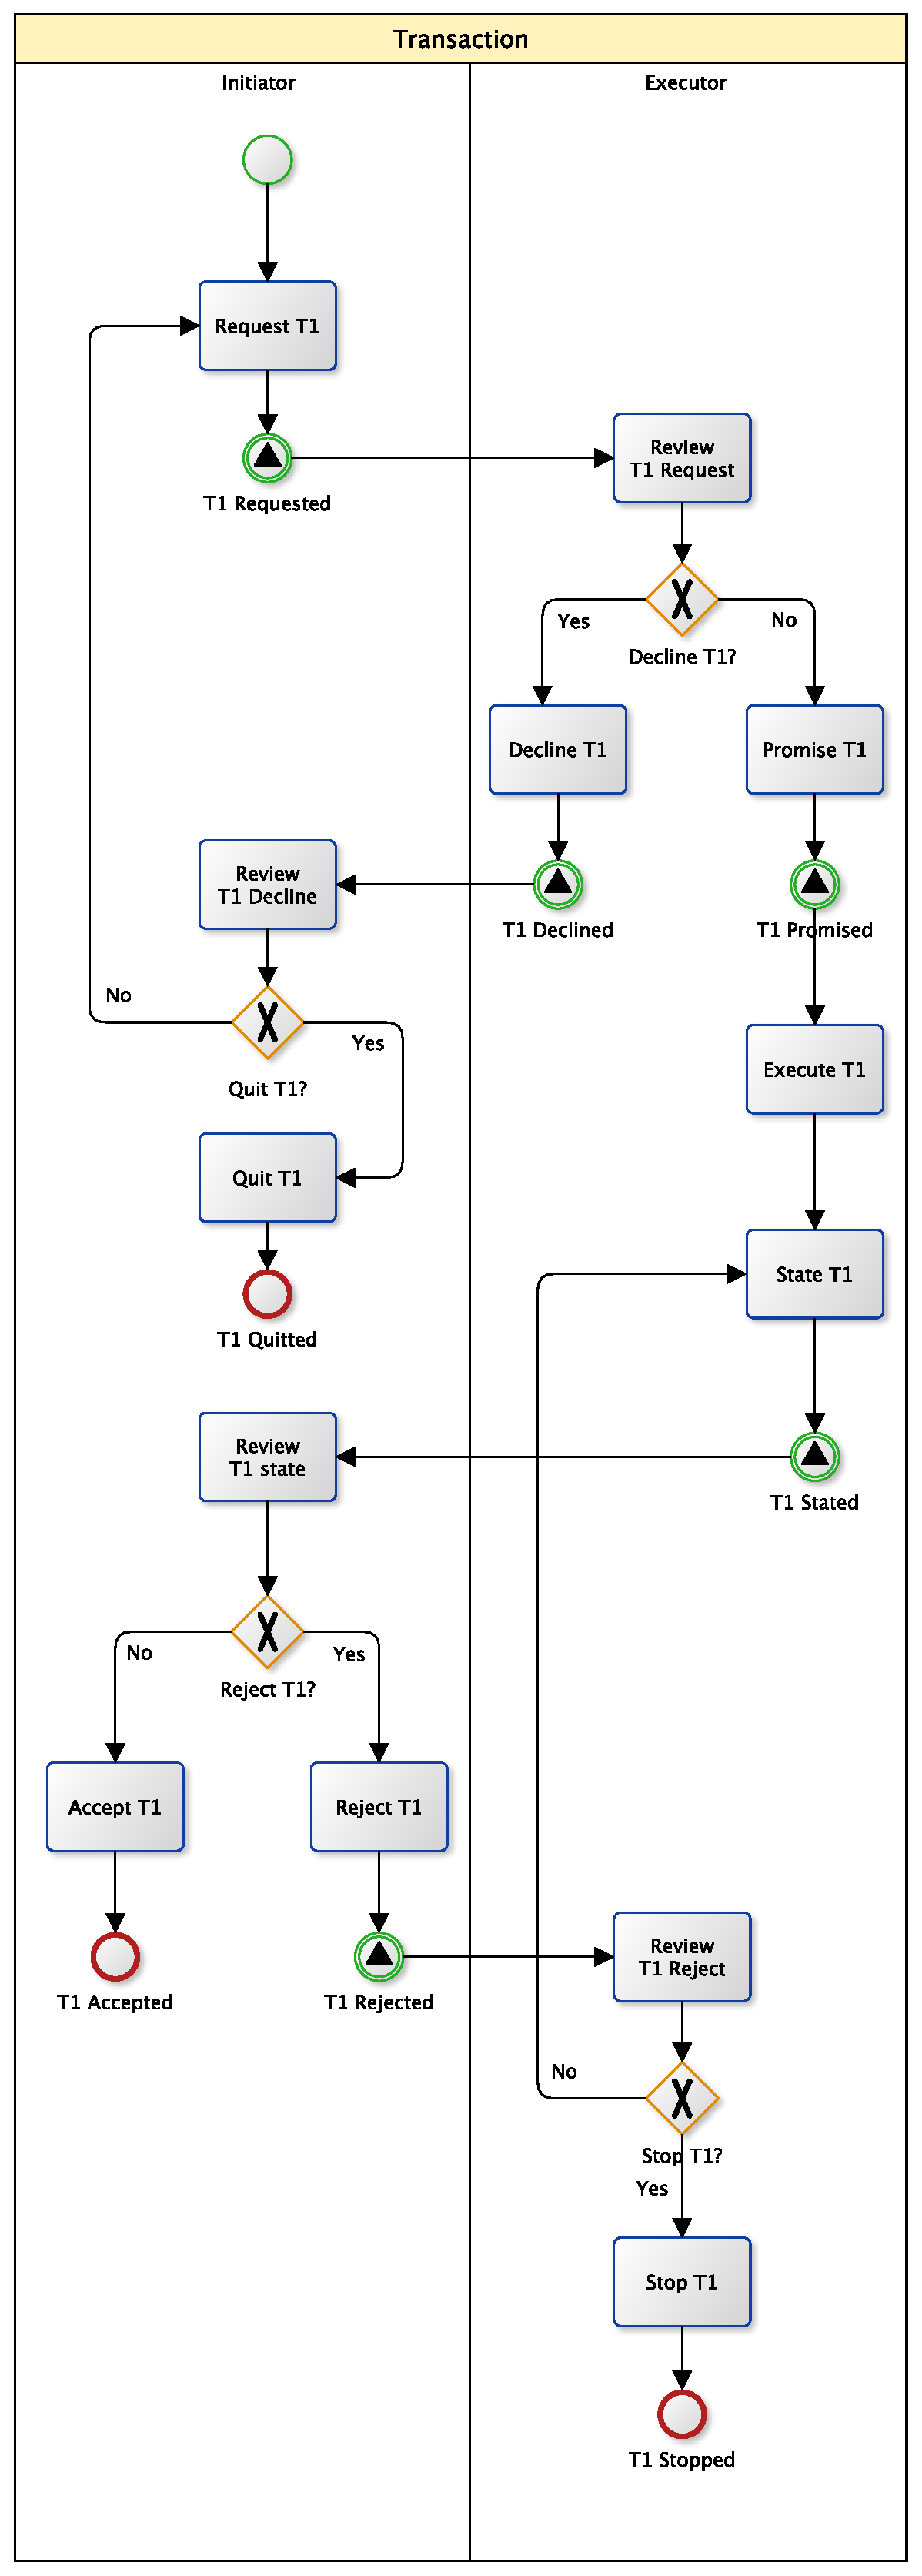
\includegraphics[width=\textwidth,height=\textheight,keepaspectratio]{obrazky/transaction-standard-signals}
\caption{Standardní transakční vzor pomocí Úloh a Signálů}
\label{fig:St_trans_ulohy_signaly}
\end{figure}

\subsection{Vyjádření pomocí Úloh a Zpráv}
Jiným přístupem k vyjádření transakčního vzoru je využít ke komunikaci mezi Actory BPMN element \textit{Zpráva}. Jelikož specifikace BPMN předepisuje, že Zpráva může být použita pouze ke komunikaci mezi \textit{Bazény}, musí být v tomto případě pro každého Actora vyhrazen zvláštní Bazén. Na obrázku \ref{fig:Zk_trans_ulohy_zpravy} lze vidět \textit{základní transakční vzor} vyjádřený tímto způsobem.

Předávání Agendy v tomto případě probíhá pomocí zaslání Zprávy a  \textit{Průběžné události (Intermediate event)}. Jakmile \textit{Actor-Initiator} provede C-act \textit{Request T1}, vyšle Zprávu reprezentující C-fact, kterou přijme \textit{Actor-Executor} na druhé straně pomocí Počáteční události typu \textit{Catch (Message)}, čímž vznikne instance procesu na straně Executora. O každém provedeném C-actu je pak druhý Actor informován pomocí Zprávy. 

V případě základního transakčního vzoru se většina problematických míst tohoto přístupu neprojevuje. K diskusi je však rozdělení Actorů do dvou Bazénů, které v podstatě znamená rozdělení transakce na dva podprocesy, jeden na straně Initiatora a jeden na straně Executora. Toto je poměrně výrazné odchýlení od transakčního axiomu tak, jak ho definuje DEMO a přináší komplikace, které se projeví v případě \textit{standardního transakčního vzoru}.

Ve standardním transakčním vzoru totiž existují místa, která při maximální snaze o dodržení standardního transakčního vzoru z DEMO mohou vyústit v deadlock. Jedná se o případy, kdy se Actor rozhodne zmamítnout výsledek C-actu \textit{Request} nebo \textit{State}. V takovém případě totiž musí Actor odpovědný za C-act rozhodnout, zda transakci zastavit nebo se pokusit o C-act znovu. Transakční vzor dle DEMO, ale nepočítá s tím, že by transakce byla rozdělena mezi dva procesy a že by měl existovat mechanismus, jak o tomto rozhodnutí informovat druhého Actora. Řešením je v tomto případě přidat do transakčního vzoru mezistavové zprávy.

V případě, že bychom nepoužili mezistavové zprávy, nastal by problém hned v případě, že by se Actor-Executor rozhodl pro \textit{Decline T1}. V takovém případě Executor vyšle zprávu Actoru-Initiatorovi a ten může buď transakci zastavit použitím \textit{Quit T1} nebo poslat \textit{Request T1} znovu. Jenže sekvenční tok v případě Executora je stále v situaci Decline T1 a bez mezistavové zprávy (neboli zprávy o rozhodnutí jak se Initiator rozhodl naložit s \textit{T1 Declined}) nemůže dále pokračovat. Částečným řešením, které můžeme vidět na obrázku \ref{fig:St_trans_ulohy_zpravy}, by v tomto případě mohlo být použít na tomto místě koncový stav T1 Declined a instanci procesu u Executora ukončit. V případě, že by se Initiator rozhodl transakci neukončit a poslal Request znovu, vznikla by nová instanci procesu na straně Executora.

Větší problém však nastane v případě, kdy by Initiator po obdržení \textit{T1 State} rozhodl tento State odmítnout a provést \textit{Reject T1}. Executor by následně obdržel zprávu o Rejectu a musel by rozhodnout, zda transakci zastavit provedením \textit{Stop T1} nebo provést \textit{State T1} znovu. Jenže bez mezistavových zpráv se Initiator nemá šanci dozvědět výsledek tohoto rozhodnutí Executora, které může být buď zastavení transakce provedením Stop T1 nebo nové provedení State. Řešení popsané v předchozím odstavci zde nebude fungovat, protože pokud by se Executor rozhodl provést znovu State T1, proces na straně Initiatora by již byl ukončen. Jediným řešením jsou tedy mezistavové zprávy, které informují druhého Actora o rozhodnutích v případě, kdy by mohlo dojít k deadlocku. Toto řešení lze vidět na obrázku \ref{fig:St_trans_ulohy_zpravy_mezistav}. Jakmile nastane Decline T1 proces na straně Executora se přesune do Průběžné události (\textit{Multiple}) a čeká na příchod mezistavové zprávy od Initiatora, jestli se rozhodl transakci ukončit nebo pošle Request znovu. Na základě toho buď proces ukončí nebo ho přesune na začátek a bude čekat na Request od Initiatora. Analogicky je pak mezistavových zpráv využito v případě State.

Využití mezistavových zpráv je však výrazným odchýlením od transakčního axiomu, protože tyto zprávy fakticky přidávají další komunikaci, se kterou transakční axiom nepočítá. Z tohoto důvodu vyhpdnocujeme tento způsob pro vyjádření transakčního axiomu jako nevhodný. 

\begin{figure}[H]\centering
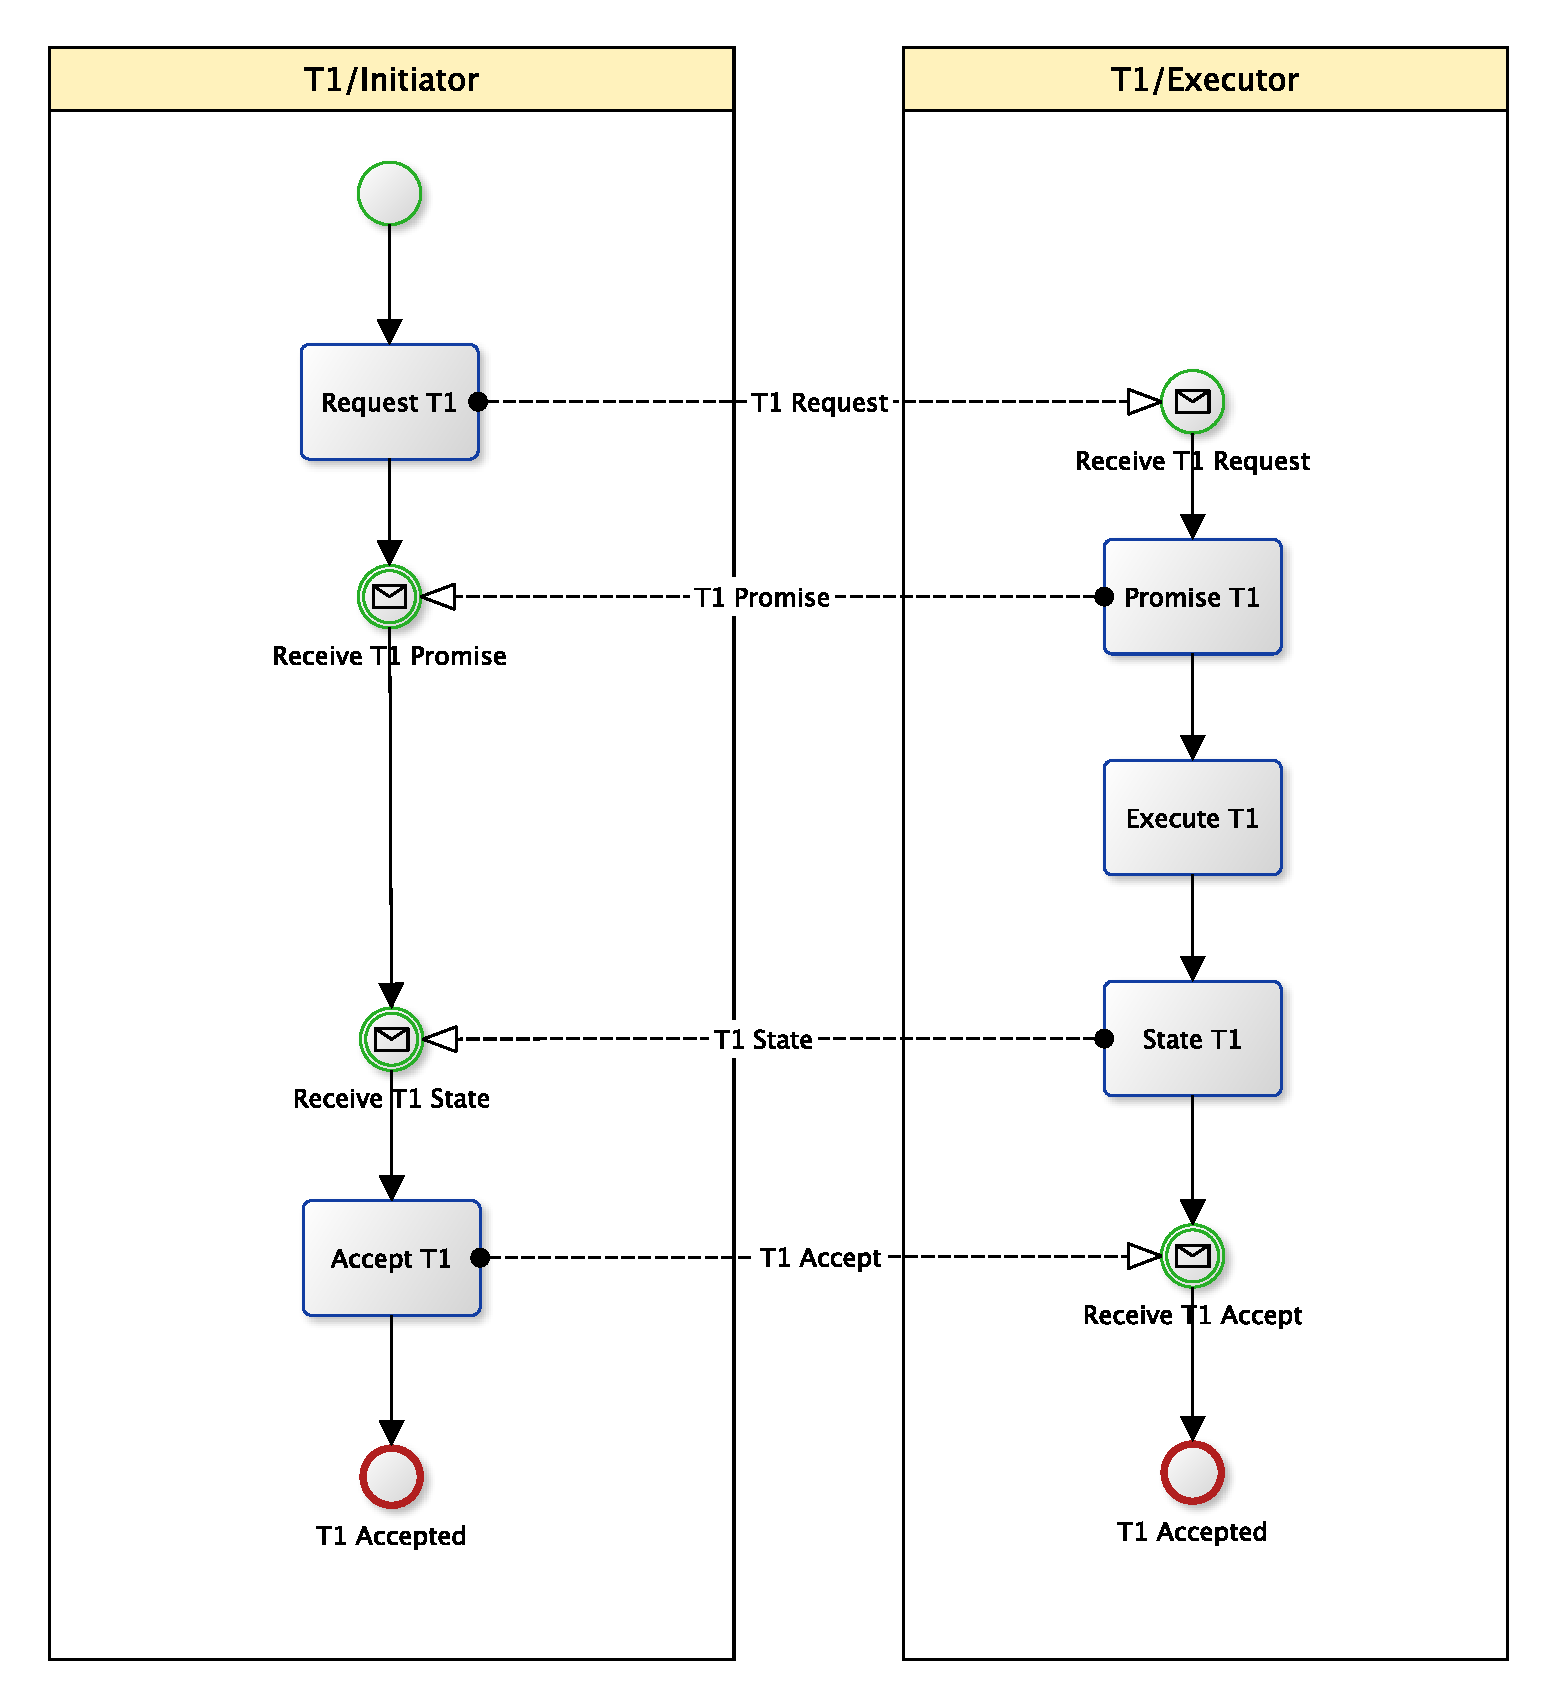
\includegraphics[width=\textwidth,height=\textheight,keepaspectratio]{obrazky/transaction-basic-messages}
\caption{Základní transakční vzor pomocí Úloh a Zpráv}
\label{fig:Zk_trans_ulohy_zpravy}
\end{figure}

\begin{figure}[H]\centering
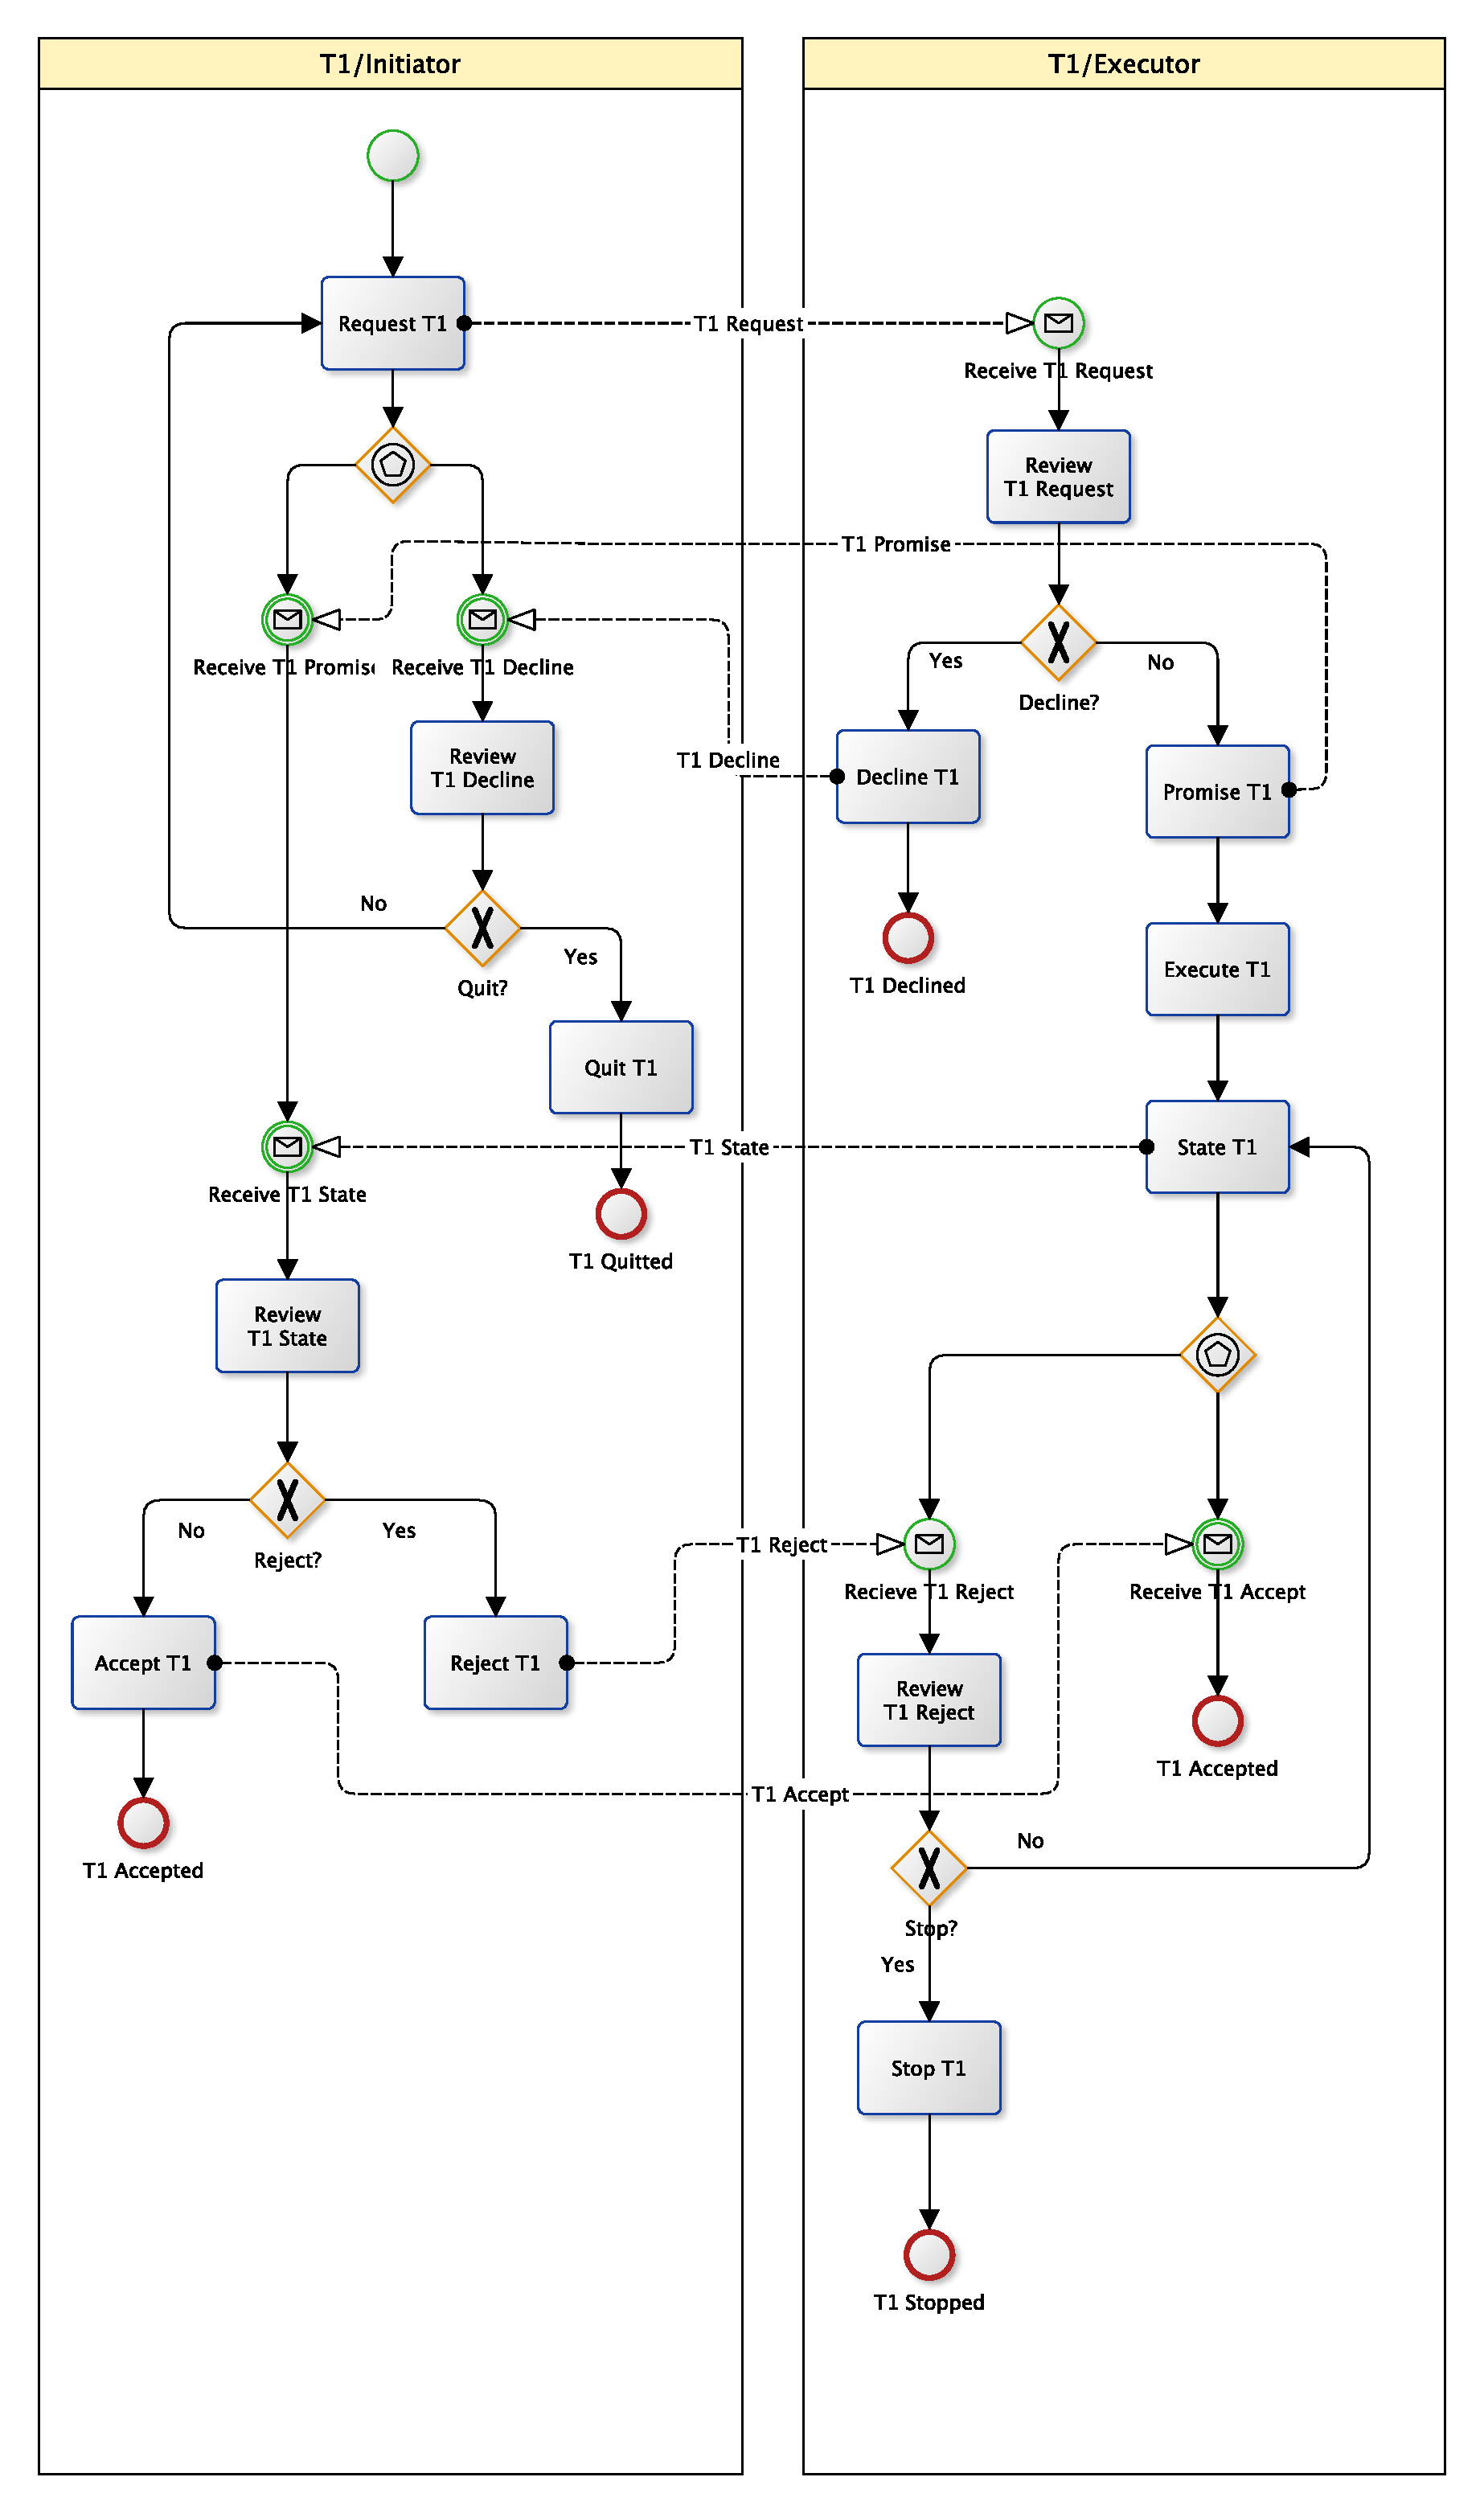
\includegraphics[width=\textwidth,height=\textheight,keepaspectratio]{obrazky/transaction-standard-messages-1}
\caption{Standardní transakční vzor pomocí Úloh a Zpráv}
\label{fig:St_trans_ulohy_zpravy}
\end{figure}

\begin{figure}[H]\centering
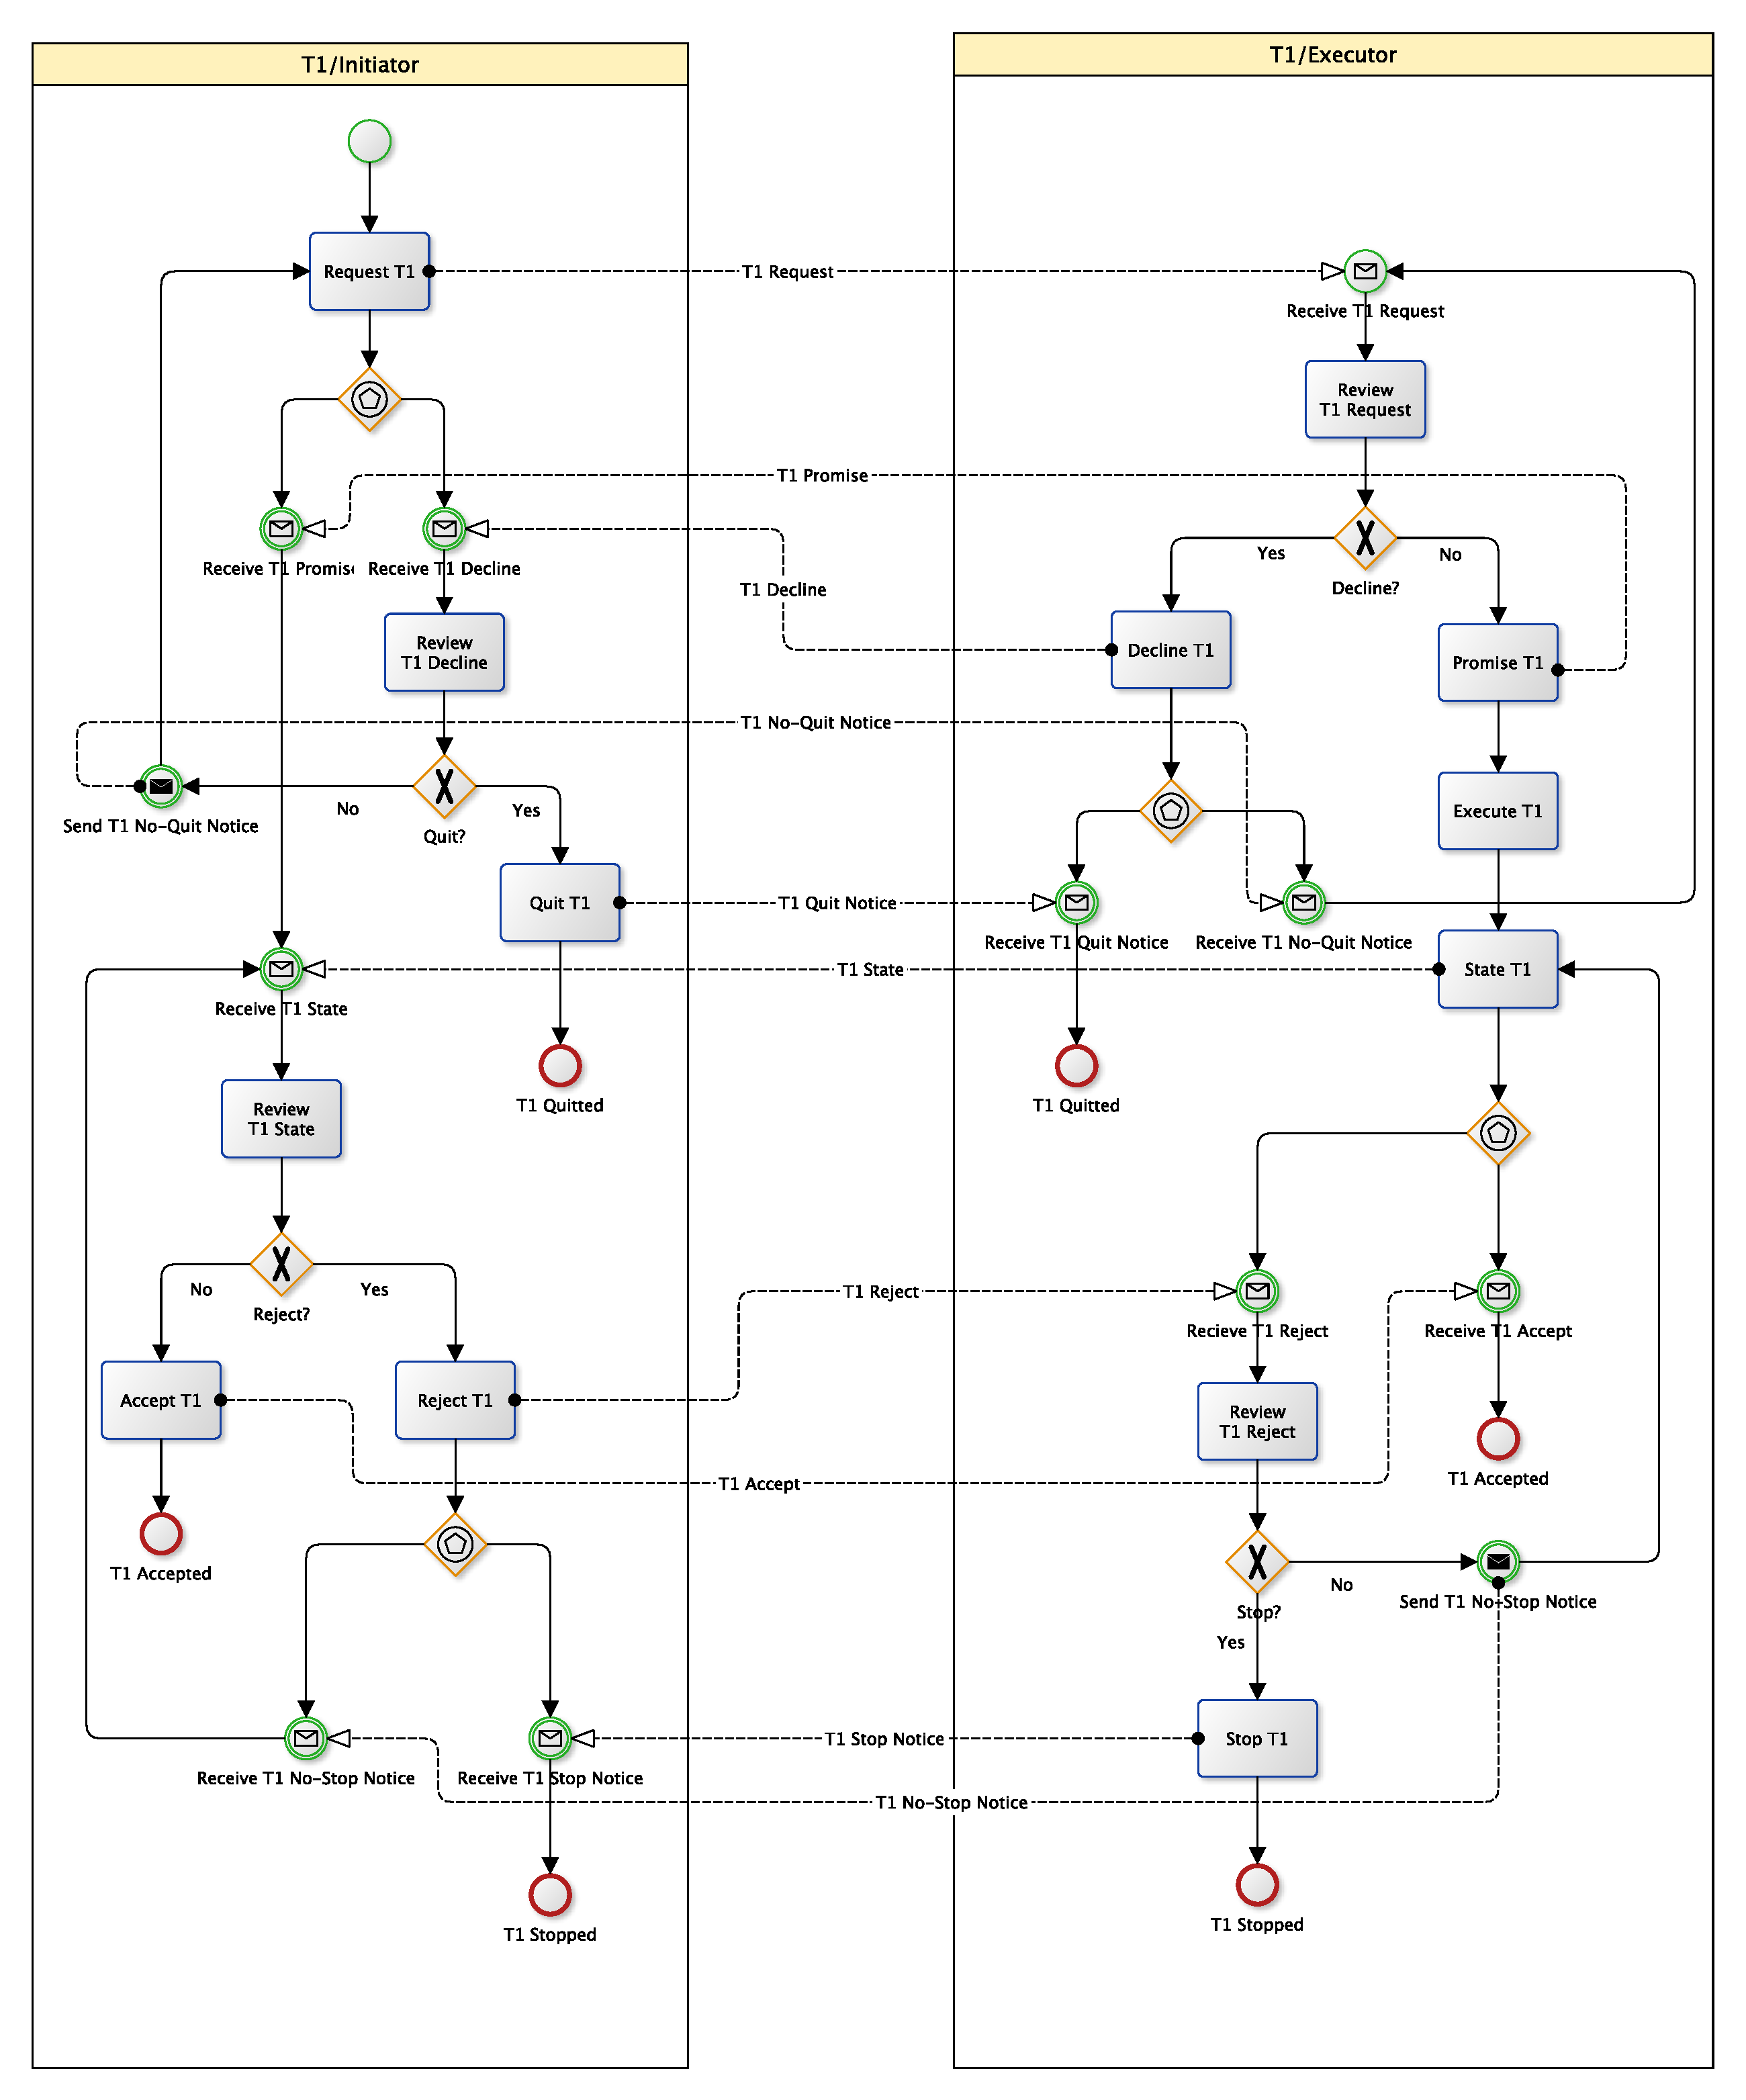
\includegraphics[width=\textwidth,height=\textheight,keepaspectratio]{obrazky/transaction-standard-messages}
\caption{Standardní transakční vzor pomocí Úloh a Zpráv (včetně mezistavových Zpráv)}
\label{fig:St_trans_ulohy_zpravy_mezistav}
\end{figure}

\section{Návrh metody pro vytváření BPMN modelů dle zásad DEMO}
V této sekci je popsána metoda pro vytváření BPMN dle zásad DEMO. Představená metoda je navržena pro vytváření zcela nových modelů, nikoli k analýze a doplnění již existujících BPMN modelů. Cílem této metody je umožnit popisovat průběh podnikových procesů v oblíbené notaci BPMN a zároveň zajistit, aby výsledný model byl \textit{kompletní} a \textit{konzistentní}.

\subsection{Předpoklady}
Aby bylo možné implementovat tuto metodu v praxi, je nezbytné, aby odpovědní pracovníci byli vybaveni následujícími teoretickými znalostmi, které vycházejí z \ptheory, Enteprise ontology a metodologie DEMO.

\begin{itemize}
\item Znalost \textit{operation axiomu} a schopnost rozlišit komunikační acty od produkčních.
\item Znalost \textit{transaction axiomu}, \textit{základního i standardního transakčního vzoru} včetně všech jeho kroků (C-actů, C-factů, P-actů, P-factů).
\item Znalost a schopnost vytvořit DEMO Actor-Transaction Diagram (ATD) a DEMO Process Structure Diagram (PSD).
\item Znalost notace BPMN včetně elementů, které oblíbená publikace \cite{Silver2011} označuje jako Level 2.
\item Znalost a schopnost aplikovat \textit{composition axiom}, tedy umět identifikovat jak jsou na sebe transakce navázané
\end{itemize}

\subsection{Krok 1: Získání textového popisu procesu}
Při vytváření modelu určitého podnikového procesu je obvyklým prvním krokem získání informací od osob, které se tohoto procesu účastní nebo mu dobře rozumí. Může se jednat o výkonné i vedoucí pracovníky a obvykle je užitečné posbírat více pohledů na jeden konkrétní proces a následně diskutovat nesrovnalosti, které mohou vzniknout.

Díky tomu, že sběr informací provádějí pracovníci se znalostí transakčního axiomu i transakčních vzorů, mohou se cíleně zeptat na jednotlivé jeho kroky. Tedy zjistit, jak probíhá \textit{request}, jak \textit{state}, jak \textit{accept} a podobně. Na konci by tedy měl vzniknout textový popis procesu s maximem relevantních informací pro další postup.

\subsection{Krok 2: Aplikace distinkčního axiomu}
Nyní jsme schopni na vzniklý textový popis procesu, chodu organizace či její složky aplikovat tzv. \textit{Performa-Informa-Forma analýzu}, což není nic jiného než praktická aplikace distinction axiomu, který je popsán v sekci \ref{sec:distinction_axiom}. Použijeme stejný postup jako v \cite{Dietz2006} a v textovém popisu označíme Performa aktivity červeně, Informa zeleně a Forma modře. Je naprosto přirozené, že u některých aktivit v textu bude problematické určit o jaký druh se jedná. S tím, jak budeme provádět další kroky dojdeme i k většímu porozumění celému procesu a je možné rozhodnutí přehodnotit. Výsledkem této části tedy je textový popis procesu s identifikovanými a vizuálně označenými Performa, Informa a Forma aktivitami.

\subsection{Krok 3: Aplikace operačního axiomu}
V tomto kroku budeme pracovat pouze s aktivitami, které jsme v Kroku 2 označili jako Performa (červeně). Úkolem je rozlišit, zda se jedná o C-act, C-fact, P-act nebo P-fact a dále k nim identifikovat příslušné actory tak jak předepisuje operation axiom. Opět není důvod nedodržet postup doporučený v \cite{Dietz2006}, tedy části textu, které indikují Actora označit hranatými závorkami \uv{[} a \uv{]}. Části textu, které indikují C-act nebo C-fact označíme kulatými závorkami \uv{(} a \uv{)}. Nakonec P-acty a P-facty nalezené v textu označíme špičatými závorkami \uv{$<$}  a \uv{$>$}. Text uzavřený v závorkách navíc podtrhneme.

\subsection{Krok 4: Zápis nalezených transakcí a jejich parametrů}
Ve čtvrtém kroku označené C-acty, C-facty, P-acty a P-facty roztřídíme dle jednotlivých \textit{transakčních kroků} (\textit{request, promise, state, accept atd.}) dle transakčního axiomu. Zároveň specifikujeme výsledek transakce a všechny poznatky učiněné v předchozích krocích zapíšeme společně do tabulky, která má strukturu dle tabulky \ref{tab:trans_param}. Navržená struktura vychází ze struktury představené v \cite{Naplava2015}.

Silnou stránkou DEMO, respektive transakčního axiomu je, že dává každé transakci (a tím i podnikovému procesu) pevně danou strukturu, kterou nelze obejít nebo upravit. I když v textovém popisu procesu nenalezneme popsané všechny transakční kroky (což se stane téměř vždy), neznamená to, že neexistují. V takovém případě je třeba jít zpět do Kroku 1 a zjistit chybějící informace od doménových a procesních vlastníků a dle nových zjištění upravit i výsledky následujících kroků metody.

\begin{table} [H] \centering
\begin{tabular}{|>{\bfseries} l| | c |}
\hline
  ID transakce & T01 \\
\hline
  Název transakce & Vyřízení objednávky $O$  \\
\hline
  Výsledek transakce & Objednávka $O$ byla vyřízena \\
\hline
  Initiator & Zákazník \\
\hline
  Executor & Mia \\
\hline
\hline
  Request & Zavolání s objednávkou \\
\hline
  Promise & Objednávka potvrzena s cenou a časem vyhotovení \\
\hline
  State & Zboží předáno zákazníkovi \\
\hline
  Accept & Zákazník odchází s balíčkem z prodejny \\
\hline
\hline
  Decline & Zamítnutí objednávky pokud zboží není na skladě \\
\hline
  Reject & \textit{chybí v popisu} \\
\hline
\hline
  Revoke request & \textit{chybí v popisu} \\
\hline
  Revoke promise & \textit{chybí v popisu} \\
\hline
  Revoke state & \textit{chybí v popisu} \\
\hline
  Revoke accept & \textit{chybí v popisu} \\
\hline
\end{tabular}
\caption{Tabulka s parametry transakce}
\label{tab:trans_param}
\end{table}

\subsection{Krok 5: Aplikace kompozičního axiomu}
Jak již bylo popsáno v \ref{sec:kompozicni_axiom} podnikový proces můžeme definovat jako množinu volně propojených transakcí. Úkolem pátého kroku je tedy identifikovat exekuce transakcí, které jsou závislé na předchozím provedení exekucí jiných transakcí. Jedinou možností jak toto prakticky provést je vrátit se k textovému popisu procesu a pokusit se identifikovat fráze, které značí závislost provádění P-actů nebo P-factů na sobě. Pokud se nám podaří objevit, že vznik P-factu B byl iniciován v průběhu vytváření P-factu A a zároveň je vznik P-factu A na B závislý, poté B je součástí A.  Všechny takto objevené závislosti zakreslíme do diagramu, který můžeme vidět na obrázku \ref{fig:result_structure_chart}.

\begin{figure}[H]\centering
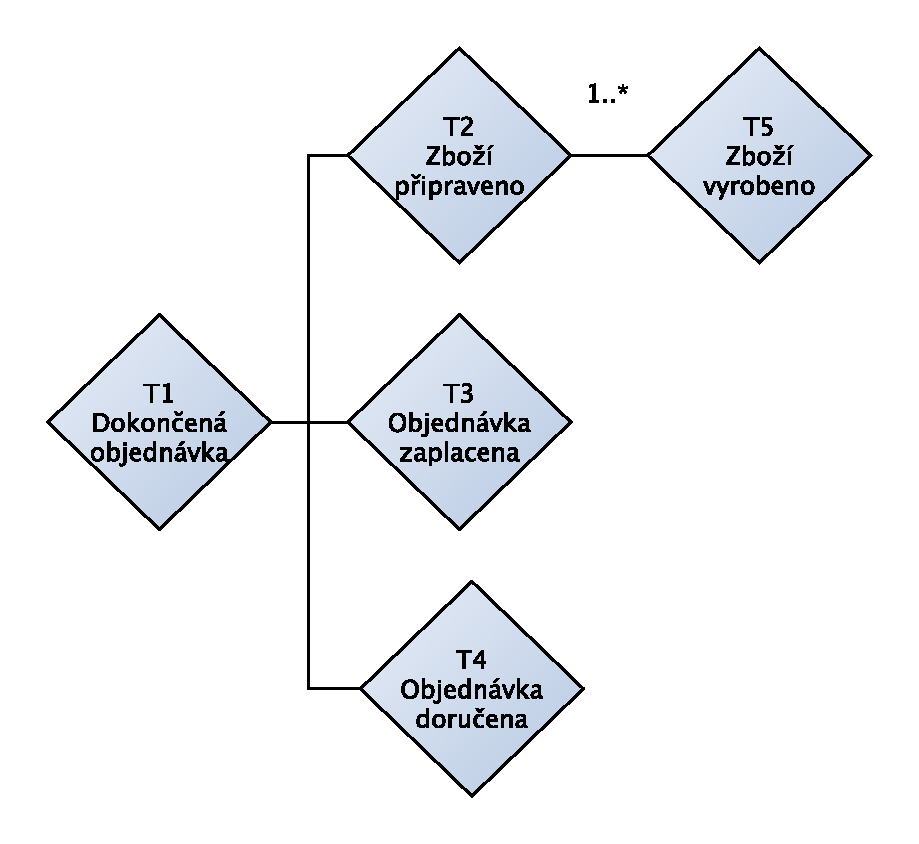
\includegraphics[width=1.0\textwidth]{obrazky/result-structure-chart}
\caption{Struktura závislosti transakcí v podnikovém procesu}
\label{fig:result_structure_chart}
\end{figure}

\subsection{Krok 6: Vytvoření DEMO modelů}
Nyní již máme dostatek informací pro vytvoření dvou DEMO modelů, které budou sloužit jako pevný bod pro verifikaci výsledného BPMN modelu i pro diskusi s byznys uživateli v případě požadavků na úpravy. Důvodem proč k této diskusi využívat DEMO modely (zejména ATD) a ne přímo výsledný BPMN model je vysoká úroveň komplexnosti BPMN modelu, který znesnadňuje jeho porozumění business uživateli.

Tabulky s popisem transakcí, které vznikly v Kroku 4 je dostatečným podkladem pro vytvoření DEMO Actor-Transaction Diagramu (ATD) i DEMO Process Structure Diagramu (PSD). ATD model zachycuje jevy v organizaci na nejvyšší úrovni abstrakce, tedy pouze actory a mezi nimi probíhající transakce. PSD jde o úroveň níže a zobrazuje jednotlivé transakční kroky stejně jako vzájemnou provázanost transakcí, kterou jsme indetifikovali v předchozím kroku. Oba modely jsou podrobně popsány v rámci kapitoly 4.

\subsection{Krok 7: Vytvoření BPMN modelu}
Nyní již máme vytvořený dostatečně silný základ a můžeme přikročit k vytvoření samotného BPMN modelu, který je výsledkem celé metody. Při jeho tvorbě využijeme zejména PSD diagram vytvořený v předchozím kroku a způsob vyjádření standardního transakčního vzoru pomocí Úloh a Signálů popsaný v sekci \ref{sec:tr_vzor_ulohy_signaly}.

Při vytváření BPMN modelu postupejeme tak, že následujeme PSD diagram od místa, kde dojde k provedení C-actu \textit{request} u kořenové transakce celého podnikového procesu a postupně převádíme jednotlivé transakční kroky do BPMN primitiv (Úloh, Signálů, Sekvenčních toků, Bran) popsaných v sekci \ref{sec:tr_vzor_ulohy_signaly}. V případě, že je podnikový proces složen z více vzájemně provázaných transakcí musíme při vytváření BPMN modelu v momentě, kdy v PSD diagramu dojdeme na místo, kde je při provedení C-actu \textit{promise} vytvořen \textit{request} na další transakci, odkloníme Sekvenční tok a pokračujeme v provádění transakčního vzoru transakce-potomka. Stejně tak pokračujeme i v dalších případech dokud se opět \uv{nevynoříme} (v případě, že všechny transakce-potomci dopadnou úspěšně) v kořenové transakci a jsme schopni provést exekuci P-actu.

V případě potřeby a pokud máme identifikované reálné aktivity příslušné k jednotlivým transakčním krokům tak můžeme tyto kroky přejmenovat i v našem výsledném BPMN modelu. %???%

1. The Perfoma-Informa-Forma Analysis. In this step all available pieces of knowledge are divided in three sets, according to the dis- tinction axiom (Chap. 12). As we will see, this is not always an easy job, since in natural language descriptions words and sentences may belong to more than one of these sets.
2. The Coordination-Actors-Production Analysis. The Performa items are divided into C-acts/results, P-acts/results, and actor roles, accord- ing to the operation axiom (Chap. 9). This step goes rather straight- forward since the three kinds are well distinguished in textual de- scriptions.

The goal of the bottom-up phase is not to translate the original model to a DEMO process model but to identify its pro- duction and coordination acts. These abstracted produc- tion and coordination acts are then modelled in DEMO and analysed according to the Ψ-theory axioms to assess their consistency and completeness.

The method starts with a BPMN process model and produces a DEMO process struc- ture diagram that abstracts the coordination and production acts depicted on the input model. The goal of the first step is to analyse the design artefacts used to represent the business process model. It analyses the activities and classifies them according to the operation axiom and distinction axiom. As a result each activity is classified as a pro- duction or coordination act (operation axiom) and also as a performa, informa, or forma speech act (distinction axiom). Furthermore, the operation axiom also discrimi- nates the actor roles involved in the process. The result of this step is a traceable list that maps the coordination and production acts and actors to the original process model from where they were sourced.
Consider the following examples: an activity that sends an electronic message is classified as a coordination act since it involves communication between actors and as a forma act because it represents a source uttering a message to a recipient. An activ- ity that archives that message is classified as forma but it is a production act because it is generating a new production fact (the archived message). An activity that counts the number of messages archived on a given date is a production act as it generates a
262 A. Caetano et al.
new production fact (the message count) but it is classified as an informa speech act since it is computing a result.
Next, each performa coordination act is classified as a request, promise, state, ac- cept coordination act according to the transaction pattern. Using the standard transac- tion pattern implies further identifying the decline, reject, stop, quit acts. . For in- stance, an activity Place Order is as a request coordination act as it is performed by the initiator to start a new transaction. The activity Receive Ordered Product is an accept coordination act as it indicates the initiator acknowledged and accepted the result of the transaction.

1.
Using the DEMO concepts provided by the three axioms,
operation axiom, construction axiom and communication axiom.
Ignore the distinction axiom, since we want to create immediately some
implementation. 

We apply an abstraction layer to reduce complexity. We capture only
communication between actors and embed production in some "production task".

Identify transactions and actors.
a single communication act identifies to some communication pattern between
who and who, and for which production etc.
If certain communication acts are not mentioned, this does not mean that they do not exist.

We have then lists of actors, transactions with communication acts and facts,
a production act and a production fact.
Using a set of well-defined BPMN primitives and constructs we can devise
a BPMN model that should be ontological complete in communication and transactions.
We abandon "happy flow only" kind of modeling.

This BPMN model is the best possible foundation for further BPMN implementation.


2.
We devise an ATD based on the actors and transaction we identified.
This an improvement, It gives a convenient useful overview, with guaranteed completeness
and much easier to analyse.
The translation to a BPMN model is now easier to do in a manual way.

Both approaches are "programming" from high level formal specifications -DEMO- using
a lower level language, BPMN / BPEL. All problems associated with normal programming 
manifest themselves. (make a list of problem manifestations and root causes, I can help)


3.
3.1 Ontological appropriateness assessment
If we are able to make a BPMN implementation of a single transaction with a reasonable
good ontological appropriateness in execution then we have made an important step.
"reasobale good" means that would "work quite good" in daily life.
Some flaws can be "quite acceptable".

3.2 Ontological truthfulness assessment
It has been proven that the DEMO models are ontological truthful and execution by the DEMO engine
is precisely compliant with the theory. 
We must show that the execution of the BPMN model is congruent with the DEMO engine
executing a DEMO model.
A lack of ontological truthfulness can be quite serious, it may invalidate all work.
If we can shown that it cannot be resolved then we have proven that BPMN cannot provide
ontological truthfulness. It is fundamentally flawed.


4.
An additional problem is exploding complexity if the number of transactions
is more than say three. Only three transactions and it explodes in a combinatorial
way in such a way that it exceeds the capabilities of normal human programmers.
It is a not-programmable system (!).

As we see DEMO models with tens of transactions in daily life this approach is much better,
but not yet good enough.

The way to address this challenge is to render BPMN models directly by the DEMO engine,
expressing in exectable BPEL.
No problem how large the BPMN models become. If BPEL is a correct formal language, not some
notation, then it should work.

The challenge is to derive some algorithm that runs through the DEMO ATD and maps DEMO
primitives to BPMN primitives and constructs, and resolves the relations between these.

Once this is clear we can build it into the DEMO engine. Should be not too difficult!

\section{Další výzkum}

Obsah této práce je prvním pokusem o vytvoření metody pro vytváření BPMN modelů podnikových procesů za použití teoretických konstruktů z \ptheory, Enterprise ontology a metodologie DEMO. Jako každá první verze i tato musí být doplněna dalším výzkumem a všechna představená východiska musí být prověřena a potvrzena.
BPMN is not a sentential language, but a graphical language, so some methodology must be found to represent graphical BPMN models in a sentential form. If we have this sentential form, then for- mal correctness can be verified using a grammar. Such a grammar is currently researched by the authors.

\nocite{*}
\bibliographystyle{plain}
\bibliography{Bibliography}

\end{document}
